% %%%%%%%%%%%%%%%%%%%%%%%%%%%%%%%%%%%%%%%%%
% \begin{frame}
% \titlepage
% \end{frame}
% %%%%%%%%%%%%%%%%%%%%%%%%%%%%%%%%%%%%%%%%%

%%%%%%%%%%%%%%%%%%%%%%%%%%%%%%%%%%%%%%%%%
\begin{frame}
\frametitle{Motivating Question}

High variation in economic performance between countries in the midst of internal armed conflict

\begin{itemize}
\item Mexico
\item India
\item Nicaragua
\end{itemize}


\end{frame}
%%%%%%%%%%%%%%%%%%%%%%%%%%%%%%%%%%%%%%%%%

%%%%%%%%%%%%%%%%%%%%%%%%%%%%%%%%%%%%%%%%%
\begin{frame}
\frametitle{Melding of Literatures}

\pause
\begin{itemize}
\item Krugman 1991; Henderson 2000; Hanson 2005 - Cities are important drivers of economic growth
\pause
\item Heterogeneity in effect of conflict on growth is due to spatial proximity of conflict relative to major urban centers
\end{itemize}

\end{frame}
%%%%%%%%%%%%%%%%%%%%%%%%%%%%%%%%%%%%%%%%%

%%%%%%%%%%%%%%%%%%%%%%%%%%%%%%%%%%%%%%%%%
\begin{frame}
\frametitle{Literature Review}

\begin{itemize}
	\item Civil War $\rightarrow$ Economic Performance
	\begin{itemize}
	\item Collier (1999) - destruction, disruption, diversion, dissaving, portfolio substitution
	% \item Imai \& Weinstein (2005) - geographical spread of conflict
	\end{itemize}
	\pause
	\item Economic Performance $\rightarrow$ Civil War
	\begin{itemize}
	% \item Collier et al. (2003) - the conflict trap
	\item Fearon \& Laitin (2003) - poor economic growth conducive for civil war
	\end{itemize}
	\pause
	\item Disaggregating Civil Wars
	\begin{itemize}
	\item Pierskalla \& Hollenbach (2013) - cell phone coverage $\rightarrow$ rebel mobilization
	\end{itemize}
\end{itemize}

\end{frame}
%%%%%%%%%%%%%%%%%%%%%%%%%%%%%%%%%%%%%%%%%

%%%%%%%%%%%%%%%%%%%%%%%%%%%%%%%%%%%%%%%%%
\begin{frame}
\frametitle{Cities, Conflict, \& Growth}

\begin{itemize}
	\item Cities $\rightarrow$ Growth
	\begin{itemize}
	\item Marshall (1920) - geographic clustering promotes valuable learning and exchange between actors
	\pause
	\item Lucas (1998) \& Glaeser et al. (1992) - accumulation of human capital generates positive spillovers
	\pause
	\item Venables (2005) - economy consists of ``lumps'' of productivity and swaths of areas contributing little to growth	
	\end{itemize}
	\pause
	\item Cities \& Conflict $\rightarrow$ Growth
	\begin{itemize}
	\item Conflicts have heterogeneous effects on economic growth 
	\item Effects determined by spatial proximity to economically relevant centers such as cities
	\end{itemize}
\end{itemize}

\end{frame}
%%%%%%%%%%%%%%%%%%%%%%%%%%%%%%%%%%%%%%%%%

%%%%%%%%%%%%%%%%%%%%%%%%%%%%%%%%%%%%%%%%%
\begin{frame}
\frametitle{FARC guerillas \& the Colombian government}

\begin{quote}FARC's strategy and [beliefs have] always been to make economic pressure on both, multinational companies and the Colombian government. This has been done by attacking oil and natural gas infrastructure affecting companies such as Pacific Rubiales Energy, Oxy and Ecopetrol. For non-fuel related international companies with subsidiaries in Colombia, such as Goodyear, Nestle, Microsoft, Toyota, among others, FARC’s modus operandi was mainly racketeering, kidnappings and extortion. (Flannery 2012)\end{quote}

\end{frame}
%%%%%%%%%%%%%%%%%%%%%%%%%%%%%%%%%%%%%%%%%

%%%%%%%%%%%%%%%%%%%%%%%%%%%%%%%%%%%%%%%%%
\begin{frame}
\frametitle{Spread of Conflict: Colombia}

\vspace{-8mm}
\begin{figure}[ht]
	\centering
	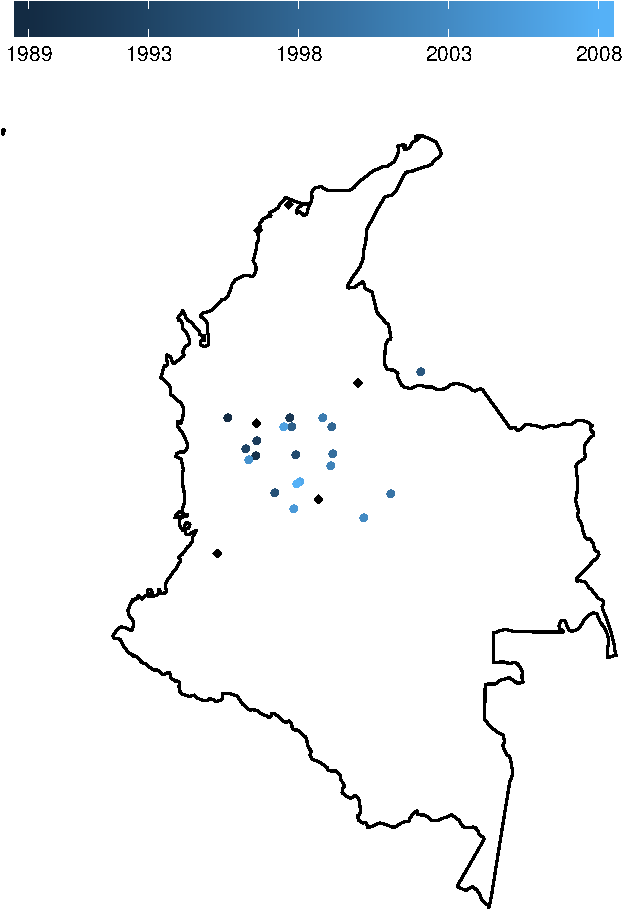
\includegraphics[width=.5\textwidth]{colombiaMap-crop}
\end{figure}

\end{frame}
%%%%%%%%%%%%%%%%%%%%%%%%%%%%%%%%%%%%%%%%%

%%%%%%%%%%%%%%%%%%%%%%%%%%%%%%%%%%%%%%%%%
\begin{frame}
\frametitle{Spread of Conflict: India}

\vspace{-8mm}
\begin{figure}[ht]
	\centering
	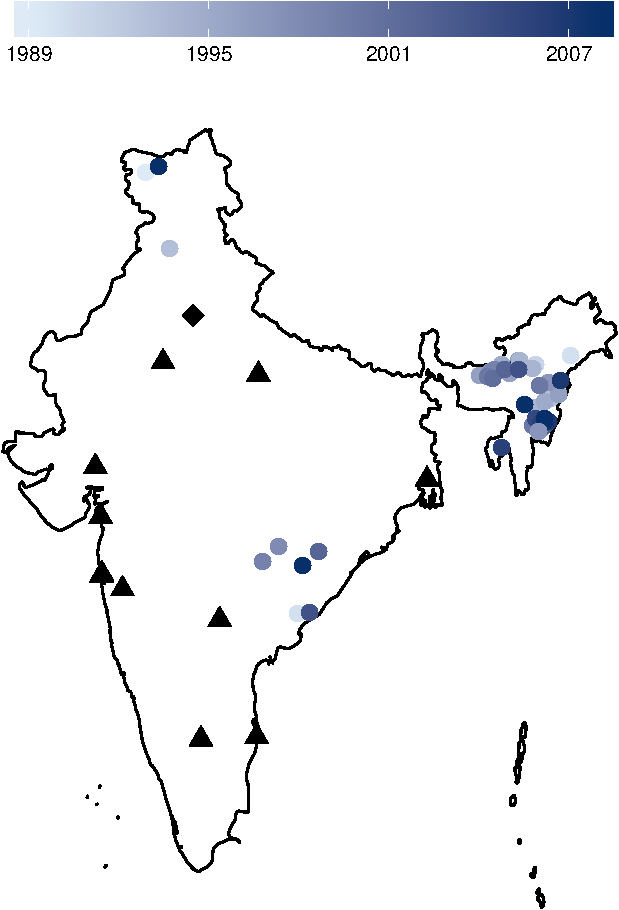
\includegraphics[width=.5\textwidth]{indiaMap-crop}
\end{figure}

\end{frame}
%%%%%%%%%%%%%%%%%%%%%%%%%%%%%%%%%%%%%%%%%

%%%%%%%%%%%%%%%%%%%%%%%%%%%%%%%%%%%%%%%%%
\begin{frame}
\frametitle{Conflict \& City Data}

% \vspace{-0.25cm}
\begin{figure}[ht]
  \centering
  % \hspace{-50mm}
  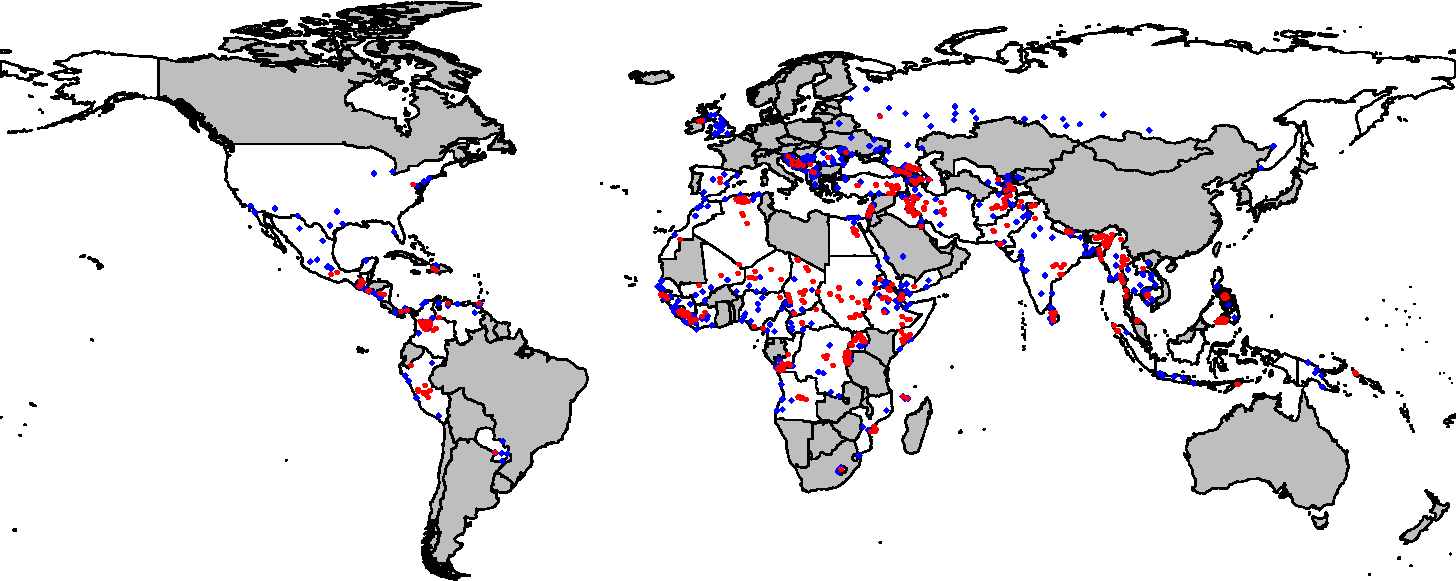
\includegraphics[width=1\textwidth]{CityConfMap-crop}
\end{figure}

\end{frame}
%%%%%%%%%%%%%%%%%%%%%%%%%%%%%%%%%%%%%%%%%

%%%%%%%%%%%%%%%%%%%%%%%%%%%%%%%%%%%%%%%%%
\begin{frame}
\frametitle{Bivariate Relationship?}

\vspace{-0.25cm}
\begin{figure}[ht]
  \centering
  \resizebox{1\textwidth}{!}{% Created by tikzDevice version 0.7.0 on 2014-10-06 19:44:25
% !TEX encoding = UTF-8 Unicode
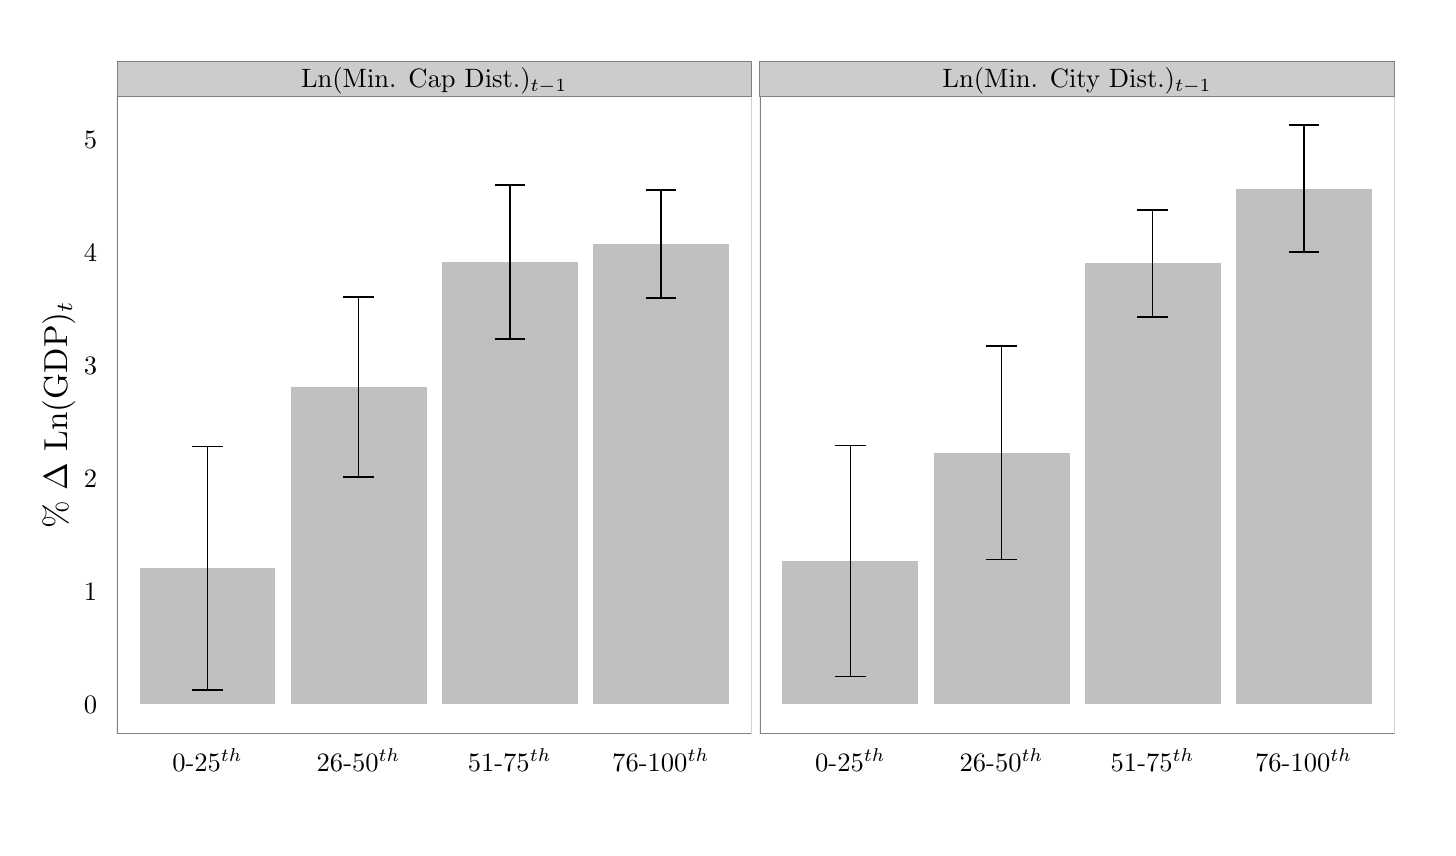
\begin{tikzpicture}[x=1pt,y=1pt]
\definecolor[named]{fillColor}{rgb}{1.00,1.00,1.00}
\path[use as bounding box,fill=fillColor,fill opacity=0.00] (0,0) rectangle (505.89,289.08);
\begin{scope}
\path[clip] (  0.00,  0.00) rectangle (505.89,289.08);
\definecolor[named]{drawColor}{rgb}{1.00,1.00,1.00}
\definecolor[named]{fillColor}{rgb}{1.00,1.00,1.00}

\path[draw=drawColor,line width= 0.6pt,line join=round,line cap=round,fill=fillColor] (  0.00,  0.00) rectangle (505.89,289.08);
\end{scope}
\begin{scope}
\path[clip] ( 32.22, 34.03) rectangle (261.53,264.40);
\definecolor[named]{fillColor}{rgb}{1.00,1.00,1.00}

\path[fill=fillColor] ( 32.22, 34.03) rectangle (261.53,264.40);
\definecolor[named]{fillColor}{rgb}{0.75,0.75,0.75}

\path[fill=fillColor] ( 40.41, 44.51) rectangle ( 89.55, 93.75);

\path[fill=fillColor] ( 95.01, 44.51) rectangle (144.14,159.24);

\path[fill=fillColor] (149.60, 44.51) rectangle (198.74,204.41);

\path[fill=fillColor] (204.20, 44.51) rectangle (253.34,210.90);
\definecolor[named]{drawColor}{rgb}{0.00,0.00,0.00}

\path[draw=drawColor,line width= 0.6pt,line join=round] ( 59.52,137.78) --
	( 70.44,137.78);

\path[draw=drawColor,line width= 0.6pt,line join=round] ( 64.98,137.78) --
	( 64.98, 49.72);

\path[draw=drawColor,line width= 0.6pt,line join=round] ( 59.52, 49.72) --
	( 70.44, 49.72);

\path[draw=drawColor,line width= 0.6pt,line join=round] (114.12,191.72) --
	(125.04,191.72);

\path[draw=drawColor,line width= 0.6pt,line join=round] (119.58,191.72) --
	(119.58,126.77);

\path[draw=drawColor,line width= 0.6pt,line join=round] (114.12,126.77) --
	(125.04,126.77);

\path[draw=drawColor,line width= 0.6pt,line join=round] (168.71,232.19) --
	(179.63,232.19);

\path[draw=drawColor,line width= 0.6pt,line join=round] (174.17,232.19) --
	(174.17,176.63);

\path[draw=drawColor,line width= 0.6pt,line join=round] (168.71,176.63) --
	(179.63,176.63);

\path[draw=drawColor,line width= 0.6pt,line join=round] (223.31,230.44) --
	(234.23,230.44);

\path[draw=drawColor,line width= 0.6pt,line join=round] (228.77,230.44) --
	(228.77,191.36);

\path[draw=drawColor,line width= 0.6pt,line join=round] (223.31,191.36) --
	(234.23,191.36);
\definecolor[named]{drawColor}{rgb}{0.50,0.50,0.50}

\path[draw=drawColor,line width= 0.6pt,line join=round,line cap=round] ( 32.22, 34.03) rectangle (261.53,264.40);
\end{scope}
\begin{scope}
\path[clip] (264.54, 34.03) rectangle (493.85,264.40);
\definecolor[named]{fillColor}{rgb}{1.00,1.00,1.00}

\path[fill=fillColor] (264.54, 34.03) rectangle (493.85,264.40);
\definecolor[named]{fillColor}{rgb}{0.75,0.75,0.75}

\path[fill=fillColor] (272.73, 44.51) rectangle (321.87, 96.35);

\path[fill=fillColor] (327.33, 44.51) rectangle (376.46,135.46);

\path[fill=fillColor] (381.92, 44.51) rectangle (431.06,203.89);

\path[fill=fillColor] (436.52, 44.51) rectangle (485.66,230.96);
\definecolor[named]{drawColor}{rgb}{0.00,0.00,0.00}

\path[draw=drawColor,line width= 0.6pt,line join=round] (291.84,138.07) --
	(302.76,138.07);

\path[draw=drawColor,line width= 0.6pt,line join=round] (297.30,138.07) --
	(297.30, 54.63);

\path[draw=drawColor,line width= 0.6pt,line join=round] (291.84, 54.63) --
	(302.76, 54.63);

\path[draw=drawColor,line width= 0.6pt,line join=round] (346.43,174.04) --
	(357.35,174.04);

\path[draw=drawColor,line width= 0.6pt,line join=round] (351.89,174.04) --
	(351.89, 96.87);

\path[draw=drawColor,line width= 0.6pt,line join=round] (346.43, 96.87) --
	(357.35, 96.87);

\path[draw=drawColor,line width= 0.6pt,line join=round] (401.03,223.16) --
	(411.95,223.16);

\path[draw=drawColor,line width= 0.6pt,line join=round] (406.49,223.16) --
	(406.49,184.61);

\path[draw=drawColor,line width= 0.6pt,line join=round] (401.03,184.61) --
	(411.95,184.61);

\path[draw=drawColor,line width= 0.6pt,line join=round] (455.63,253.93) --
	(466.55,253.93);

\path[draw=drawColor,line width= 0.6pt,line join=round] (461.09,253.93) --
	(461.09,208.00);

\path[draw=drawColor,line width= 0.6pt,line join=round] (455.63,208.00) --
	(466.55,208.00);
\definecolor[named]{drawColor}{rgb}{0.50,0.50,0.50}

\path[draw=drawColor,line width= 0.6pt,line join=round,line cap=round] (264.54, 34.03) rectangle (493.85,264.40);
\end{scope}
\begin{scope}
\path[clip] (  0.00,  0.00) rectangle (505.89,289.08);
\definecolor[named]{drawColor}{rgb}{0.50,0.50,0.50}
\definecolor[named]{fillColor}{rgb}{0.80,0.80,0.80}

\path[draw=drawColor,line width= 0.2pt,line join=round,line cap=round,fill=fillColor] ( 32.22,264.40) rectangle (261.53,277.04);
\definecolor[named]{drawColor}{rgb}{0.00,0.00,0.00}

\node[text=drawColor,anchor=base,inner sep=0pt, outer sep=0pt, scale=  0.96] at (146.87,267.41) {Ln(Min. Cap Dist.)$_{t-1}$};
\end{scope}
\begin{scope}
\path[clip] (  0.00,  0.00) rectangle (505.89,289.08);
\definecolor[named]{drawColor}{rgb}{0.50,0.50,0.50}
\definecolor[named]{fillColor}{rgb}{0.80,0.80,0.80}

\path[draw=drawColor,line width= 0.2pt,line join=round,line cap=round,fill=fillColor] (264.54,264.40) rectangle (493.85,277.04);
\definecolor[named]{drawColor}{rgb}{0.00,0.00,0.00}

\node[text=drawColor,anchor=base,inner sep=0pt, outer sep=0pt, scale=  0.96] at (379.19,267.41) {Ln(Min. City Dist.)$_{t-1}$};
\end{scope}
\begin{scope}
\path[clip] (  0.00,  0.00) rectangle (505.89,289.08);
\definecolor[named]{drawColor}{rgb}{0.00,0.00,0.00}

\node[text=drawColor,anchor=base east,inner sep=0pt, outer sep=0pt, scale=  0.96] at ( 25.11, 41.20) {0};

\node[text=drawColor,anchor=base east,inner sep=0pt, outer sep=0pt, scale=  0.96] at ( 25.11, 82.02) {1};

\node[text=drawColor,anchor=base east,inner sep=0pt, outer sep=0pt, scale=  0.96] at ( 25.11,122.84) {2};

\node[text=drawColor,anchor=base east,inner sep=0pt, outer sep=0pt, scale=  0.96] at ( 25.11,163.67) {3};

\node[text=drawColor,anchor=base east,inner sep=0pt, outer sep=0pt, scale=  0.96] at ( 25.11,204.49) {4};

\node[text=drawColor,anchor=base east,inner sep=0pt, outer sep=0pt, scale=  0.96] at ( 25.11,245.31) {5};
\end{scope}
\begin{scope}
\path[clip] (  0.00,  0.00) rectangle (505.89,289.08);
\definecolor[named]{drawColor}{rgb}{0.00,0.00,0.00}

\node[text=drawColor,anchor=base,inner sep=0pt, outer sep=0pt, scale=  0.96] at ( 64.98, 20.31) {0-25$^{th}$};

\node[text=drawColor,anchor=base,inner sep=0pt, outer sep=0pt, scale=  0.96] at (119.58, 20.31) {26-50$^{th}$};

\node[text=drawColor,anchor=base,inner sep=0pt, outer sep=0pt, scale=  0.96] at (174.17, 20.31) {51-75$^{th}$};

\node[text=drawColor,anchor=base,inner sep=0pt, outer sep=0pt, scale=  0.96] at (228.77, 20.31) {76-100$^{th}$};
\end{scope}
\begin{scope}
\path[clip] (  0.00,  0.00) rectangle (505.89,289.08);
\definecolor[named]{drawColor}{rgb}{0.00,0.00,0.00}

\node[text=drawColor,anchor=base,inner sep=0pt, outer sep=0pt, scale=  0.96] at (297.30, 20.31) {0-25$^{th}$};

\node[text=drawColor,anchor=base,inner sep=0pt, outer sep=0pt, scale=  0.96] at (351.89, 20.31) {26-50$^{th}$};

\node[text=drawColor,anchor=base,inner sep=0pt, outer sep=0pt, scale=  0.96] at (406.49, 20.31) {51-75$^{th}$};

\node[text=drawColor,anchor=base,inner sep=0pt, outer sep=0pt, scale=  0.96] at (461.09, 20.31) {76-100$^{th}$};
\end{scope}
\begin{scope}
\path[clip] (  0.00,  0.00) rectangle (505.89,289.08);
\definecolor[named]{drawColor}{rgb}{0.00,0.00,0.00}

\node[text=drawColor,rotate= 90.00,anchor=base,inner sep=0pt, outer sep=0pt, scale=  1.20] at ( 14.29,149.22) {\% $\Delta$ Ln(GDP)$_{t}$};
\end{scope}
\end{tikzpicture}
}
\end{figure}

\end{frame}
%%%%%%%%%%%%%%%%%%%%%%%%%%%%%%%%%%%%%%%%%

%%%%%%%%%%%%%%%%%%%%%%%%%%%%%%%%%%%%%%%%%
\begin{frame}
\frametitle{Estimation Approach}

\begin{align*}
	\% \Delta Ln(GDP)_{i,t} &= \beta_{1}(Ln(Min. \; Conflict \; Dist.)_{i,t-1}) \\
	& \;+\; \beta_{2}(Conflict \; Intensity_{i,t-1}) \\
	& \;+\; \beta_{3}(Conflict \; Duration_{i,t-1}) \\
	& \;+\; \beta_{4}(Conflict \; Area_{i,t-1} \;/\; Land \; Area_{i,t-1} > 50\%) \\
	& \;+\; \beta_{5}(Number \; of \; Conflicts_{i,t-1}) \\
	& \;+\; \beta_{6}(Upper \; Income_{i,t}) \\	
	& \;+\; \beta_{7}(Inflation_{i,t-1}) \;+\; \beta_{8}(Democracy_{i,t-1}) \\
	& \;+\; \beta_{9}(Resource \; Rents/GDP_{t-1}) \\ 
	& \;+\; \beta_{10}(World \; GDP \; Growth_{t}) \;+\; \mu_{i,t} \;+\; \epsilon_{i,t}
\end{align*}

\end{frame}
%%%%%%%%%%%%%%%%%%%%%%%%%%%%%%%%%%%%%%%%%

%%%%%%%%%%%%%%%%%%%%%%%%%%%%%%%%%%%%%%%%%
\begin{frame}
\frametitle{Findings}

\vspace{-8mm}
\begin{figure}
	\centering
	\begin{tabular}{cc}
	\hspace{-9mm}
		\resizebox{.5\textwidth}{!}{% Created by tikzDevice version 0.8.1 on 2015-08-25 14:10:34
% !TEX encoding = UTF-8 Unicode
\begin{tikzpicture}[x=1pt,y=1pt]
\definecolor{fillColor}{RGB}{255,255,255}
\path[use as bounding box,fill=fillColor,fill opacity=0.00] (0,0) rectangle (289.08,433.62);
\begin{scope}
\path[clip] (  0.00,  0.00) rectangle (289.08,433.62);
\definecolor{drawColor}{RGB}{255,255,255}
\definecolor{fillColor}{RGB}{255,255,255}

\path[draw=drawColor,line width= 0.6pt,line join=round,line cap=round,fill=fillColor] ( -0.00,  0.00) rectangle (289.08,433.62);
\end{scope}
\begin{scope}
\path[clip] (137.46, 34.03) rectangle (277.03,421.57);
\definecolor{fillColor}{RGB}{255,255,255}

\path[fill=fillColor] (137.46, 34.03) rectangle (277.03,421.57);
\definecolor{drawColor}{RGB}{54,144,192}

\path[draw=drawColor,draw opacity=0.30,line width= 0.3pt,line join=round] (213.47, 56.83) -- (223.69, 56.83);

\path[draw=drawColor,draw opacity=0.30,line width= 0.3pt,line join=round] (213.37, 94.83) -- (214.72, 94.83);
\definecolor{drawColor}{RGB}{150,150,150}

\path[draw=drawColor,draw opacity=0.30,line width= 0.3pt,line join=round] (211.43,132.82) -- (214.83,132.82);
\definecolor{drawColor}{RGB}{222,45,38}

\path[draw=drawColor,draw opacity=0.30,line width= 0.3pt,line join=round] (179.19,170.81) -- (196.84,170.81);
\definecolor{drawColor}{RGB}{150,150,150}

\path[draw=drawColor,draw opacity=0.30,line width= 0.3pt,line join=round] (169.39,208.81) -- (270.69,208.81);
\definecolor{drawColor}{RGB}{54,144,192}

\path[draw=drawColor,draw opacity=0.30,line width= 0.3pt,line join=round] (215.48,246.80) -- (238.71,246.80);
\definecolor{drawColor}{RGB}{222,45,38}

\path[draw=drawColor,draw opacity=0.30,line width= 0.3pt,line join=round] (143.80,284.80) -- (192.56,284.80);
\definecolor{drawColor}{RGB}{54,144,192}

\path[draw=drawColor,draw opacity=0.30,line width= 0.3pt,line join=round] (214.05,322.79) -- (215.43,322.79);
\definecolor{drawColor}{RGB}{150,150,150}

\path[draw=drawColor,draw opacity=0.30,line width= 0.3pt,line join=round] (184.07,360.78) -- (220.64,360.78);
\definecolor{drawColor}{RGB}{54,144,192}

\path[draw=drawColor,draw opacity=0.30,line width= 0.3pt,line join=round] (215.48,398.78) -- (230.32,398.78);
\definecolor{drawColor}{RGB}{54,144,192}

\path[draw=drawColor,line width= 1.1pt,line join=round] (214.29, 56.83) -- (222.87, 56.83);

\path[draw=drawColor,line width= 1.1pt,line join=round] (213.48, 94.83) -- (214.61, 94.83);
\definecolor{drawColor}{gray}{0.59}

\path[draw=drawColor,line width= 1.1pt,line join=round] (211.71,132.82) -- (214.56,132.82);
\definecolor{drawColor}{RGB}{222,45,38}

\path[draw=drawColor,line width= 1.1pt,line join=round] (180.61,170.81) -- (195.42,170.81);
\definecolor{drawColor}{gray}{0.59}

\path[draw=drawColor,line width= 1.1pt,line join=round] (177.53,208.81) -- (262.55,208.81);
\definecolor{drawColor}{RGB}{54,144,192}

\path[draw=drawColor,line width= 1.1pt,line join=round] (217.35,246.80) -- (236.85,246.80);
\definecolor{drawColor}{RGB}{222,45,38}

\path[draw=drawColor,line width= 1.1pt,line join=round] (147.72,284.80) -- (188.64,284.80);
\definecolor{drawColor}{RGB}{54,144,192}

\path[draw=drawColor,line width= 1.1pt,line join=round] (214.16,322.79) -- (215.32,322.79);
\definecolor{drawColor}{gray}{0.59}

\path[draw=drawColor,line width= 1.1pt,line join=round] (187.01,360.78) -- (217.70,360.78);
\definecolor{drawColor}{RGB}{54,144,192}

\path[draw=drawColor,line width= 1.1pt,line join=round] (216.67,398.78) -- (229.13,398.78);
\definecolor{drawColor}{RGB}{0,0,0}

\path[draw=drawColor,line width= 0.6pt,dash pattern=on 4pt off 4pt ,line join=round] (213.36, 34.03) -- (213.36,421.57);
\definecolor{drawColor}{RGB}{54,144,192}
\definecolor{fillColor}{RGB}{54,144,192}

\path[draw=drawColor,line width= 0.4pt,line join=round,line cap=round,fill=fillColor] (222.90,398.78) circle (  2.85);
\definecolor{drawColor}{gray}{0.59}
\definecolor{fillColor}{gray}{0.59}

\path[draw=drawColor,line width= 0.4pt,line join=round,line cap=round,fill=fillColor] (202.36,360.78) circle (  2.85);
\definecolor{drawColor}{RGB}{54,144,192}
\definecolor{fillColor}{RGB}{54,144,192}

\path[draw=drawColor,line width= 0.4pt,line join=round,line cap=round,fill=fillColor] (214.74,322.79) circle (  2.85);
\definecolor{drawColor}{RGB}{222,45,38}
\definecolor{fillColor}{RGB}{222,45,38}

\path[draw=drawColor,line width= 0.4pt,line join=round,line cap=round,fill=fillColor] (168.18,284.80) circle (  2.85);
\definecolor{drawColor}{RGB}{54,144,192}
\definecolor{fillColor}{RGB}{54,144,192}

\path[draw=drawColor,line width= 0.4pt,line join=round,line cap=round,fill=fillColor] (227.10,246.80) circle (  2.85);
\definecolor{drawColor}{gray}{0.59}
\definecolor{fillColor}{gray}{0.59}

\path[draw=drawColor,line width= 0.4pt,line join=round,line cap=round,fill=fillColor] (220.04,208.81) circle (  2.85);
\definecolor{drawColor}{RGB}{222,45,38}
\definecolor{fillColor}{RGB}{222,45,38}

\path[draw=drawColor,line width= 0.4pt,line join=round,line cap=round,fill=fillColor] (188.02,170.81) circle (  2.85);
\definecolor{drawColor}{gray}{0.59}
\definecolor{fillColor}{gray}{0.59}

\path[draw=drawColor,line width= 0.4pt,line join=round,line cap=round,fill=fillColor] (213.13,132.82) circle (  2.85);
\definecolor{drawColor}{RGB}{54,144,192}
\definecolor{fillColor}{RGB}{54,144,192}

\path[draw=drawColor,line width= 0.4pt,line join=round,line cap=round,fill=fillColor] (214.05, 94.83) circle (  2.85);

\path[draw=drawColor,line width= 0.4pt,line join=round,line cap=round,fill=fillColor] (218.58, 56.83) circle (  2.85);

\path[draw=drawColor,line width= 0.6pt,line join=round] (223.69, 54.93) --
	(223.69, 58.73);

\path[draw=drawColor,line width= 0.6pt,line join=round] (223.69, 56.83) --
	(213.47, 56.83);

\path[draw=drawColor,line width= 0.6pt,line join=round] (213.47, 54.93) --
	(213.47, 58.73);

\path[draw=drawColor,line width= 0.6pt,line join=round] (214.72, 92.93) --
	(214.72, 96.72);

\path[draw=drawColor,line width= 0.6pt,line join=round] (214.72, 94.83) --
	(213.37, 94.83);

\path[draw=drawColor,line width= 0.6pt,line join=round] (213.37, 92.93) --
	(213.37, 96.72);
\definecolor{drawColor}{gray}{0.59}

\path[draw=drawColor,line width= 0.6pt,line join=round] (214.83,130.92) --
	(214.83,134.72);

\path[draw=drawColor,line width= 0.6pt,line join=round] (214.83,132.82) --
	(211.43,132.82);

\path[draw=drawColor,line width= 0.6pt,line join=round] (211.43,130.92) --
	(211.43,134.72);
\definecolor{drawColor}{RGB}{222,45,38}

\path[draw=drawColor,line width= 0.6pt,line join=round] (196.84,168.91) --
	(196.84,172.71);

\path[draw=drawColor,line width= 0.6pt,line join=round] (196.84,170.81) --
	(179.19,170.81);

\path[draw=drawColor,line width= 0.6pt,line join=round] (179.19,168.91) --
	(179.19,172.71);
\definecolor{drawColor}{gray}{0.59}

\path[draw=drawColor,line width= 0.6pt,line join=round] (270.69,206.91) --
	(270.69,210.71);

\path[draw=drawColor,line width= 0.6pt,line join=round] (270.69,208.81) --
	(169.39,208.81);

\path[draw=drawColor,line width= 0.6pt,line join=round] (169.39,206.91) --
	(169.39,210.71);
\definecolor{drawColor}{RGB}{54,144,192}

\path[draw=drawColor,line width= 0.6pt,line join=round] (238.71,244.90) --
	(238.71,248.70);

\path[draw=drawColor,line width= 0.6pt,line join=round] (238.71,246.80) --
	(215.48,246.80);

\path[draw=drawColor,line width= 0.6pt,line join=round] (215.48,244.90) --
	(215.48,248.70);
\definecolor{drawColor}{RGB}{222,45,38}

\path[draw=drawColor,line width= 0.6pt,line join=round] (192.56,282.90) --
	(192.56,286.70);

\path[draw=drawColor,line width= 0.6pt,line join=round] (192.56,284.80) --
	(143.80,284.80);

\path[draw=drawColor,line width= 0.6pt,line join=round] (143.80,282.90) --
	(143.80,286.70);
\definecolor{drawColor}{RGB}{54,144,192}

\path[draw=drawColor,line width= 0.6pt,line join=round] (215.43,320.89) --
	(215.43,324.69);

\path[draw=drawColor,line width= 0.6pt,line join=round] (215.43,322.79) --
	(214.05,322.79);

\path[draw=drawColor,line width= 0.6pt,line join=round] (214.05,320.89) --
	(214.05,324.69);
\definecolor{drawColor}{gray}{0.59}

\path[draw=drawColor,line width= 0.6pt,line join=round] (220.64,358.88) --
	(220.64,362.68);

\path[draw=drawColor,line width= 0.6pt,line join=round] (220.64,360.78) --
	(184.07,360.78);

\path[draw=drawColor,line width= 0.6pt,line join=round] (184.07,358.88) --
	(184.07,362.68);
\definecolor{drawColor}{RGB}{54,144,192}

\path[draw=drawColor,line width= 0.6pt,line join=round] (230.32,396.88) --
	(230.32,400.68);

\path[draw=drawColor,line width= 0.6pt,line join=round] (230.32,398.78) --
	(215.48,398.78);

\path[draw=drawColor,line width= 0.6pt,line join=round] (215.48,396.88) --
	(215.48,400.68);
\end{scope}
\begin{scope}
\path[clip] (  0.00,  0.00) rectangle (289.08,433.62);
\definecolor{drawColor}{RGB}{0,0,0}

\path[draw=drawColor,line width= 0.6pt,line join=round] (137.46, 34.03) --
	(137.46,421.57);
\end{scope}
\begin{scope}
\path[clip] (  0.00,  0.00) rectangle (289.08,433.62);
\definecolor{drawColor}{RGB}{0,0,0}

\node[text=drawColor,anchor=base east,inner sep=0pt, outer sep=0pt, scale=  0.96] at (130.35, 53.53) {World GDP Growth$_{t}$};

\node[text=drawColor,anchor=base east,inner sep=0pt, outer sep=0pt, scale=  0.96] at (130.35, 91.52) {Resource Rents/GDP$_{t-1}$};

\node[text=drawColor,anchor=base east,inner sep=0pt, outer sep=0pt, scale=  0.96] at (130.35,129.51) {Democracy$_{t-1}$};

\node[text=drawColor,anchor=base east,inner sep=0pt, outer sep=0pt, scale=  0.96] at (130.35,167.51) {Ln(Inflation)$_{t-1}$};

\node[text=drawColor,anchor=base east,inner sep=0pt, outer sep=0pt, scale=  0.96] at (130.35,205.50) {Upper Income};

\node[text=drawColor,anchor=base east,inner sep=0pt, outer sep=0pt, scale=  0.96] at (130.35,243.50) {Number of conflicts$_{t-1}$};

\node[text=drawColor,anchor=base east,inner sep=0pt, outer sep=0pt, scale=  0.96] at (130.35,281.49) {Area$_{t-1}$};

\node[text=drawColor,anchor=base east,inner sep=0pt, outer sep=0pt, scale=  0.96] at (130.35,319.48) {Duration$_{t-1}$};

\node[text=drawColor,anchor=base east,inner sep=0pt, outer sep=0pt, scale=  0.96] at (130.35,357.48) {Intensity$_{t-1}$};

\node[text=drawColor,anchor=base east,inner sep=0pt, outer sep=0pt, scale=  0.96] at (130.35,395.47) {Ln(Min. Capital Dist.)$_{t-1}$};
\end{scope}
\begin{scope}
\path[clip] (  0.00,  0.00) rectangle (289.08,433.62);
\definecolor{drawColor}{RGB}{0,0,0}

\path[draw=drawColor,line width= 0.6pt,line join=round] (137.46, 34.03) --
	(277.03, 34.03);
\end{scope}
\begin{scope}
\path[clip] (  0.00,  0.00) rectangle (289.08,433.62);
\definecolor{drawColor}{RGB}{0,0,0}

\node[text=drawColor,anchor=base,inner sep=0pt, outer sep=0pt, scale=  0.96] at (174.95, 20.31) {-4};

\node[text=drawColor,anchor=base,inner sep=0pt, outer sep=0pt, scale=  0.96] at (213.36, 20.31) {0};

\node[text=drawColor,anchor=base,inner sep=0pt, outer sep=0pt, scale=  0.96] at (251.77, 20.31) {4};
\end{scope}
\end{tikzpicture}
} &
		\resizebox{.5\textwidth}{!}{% Created by tikzDevice version 0.7.0 on 2014-09-25 14:01:51
% !TEX encoding = UTF-8 Unicode
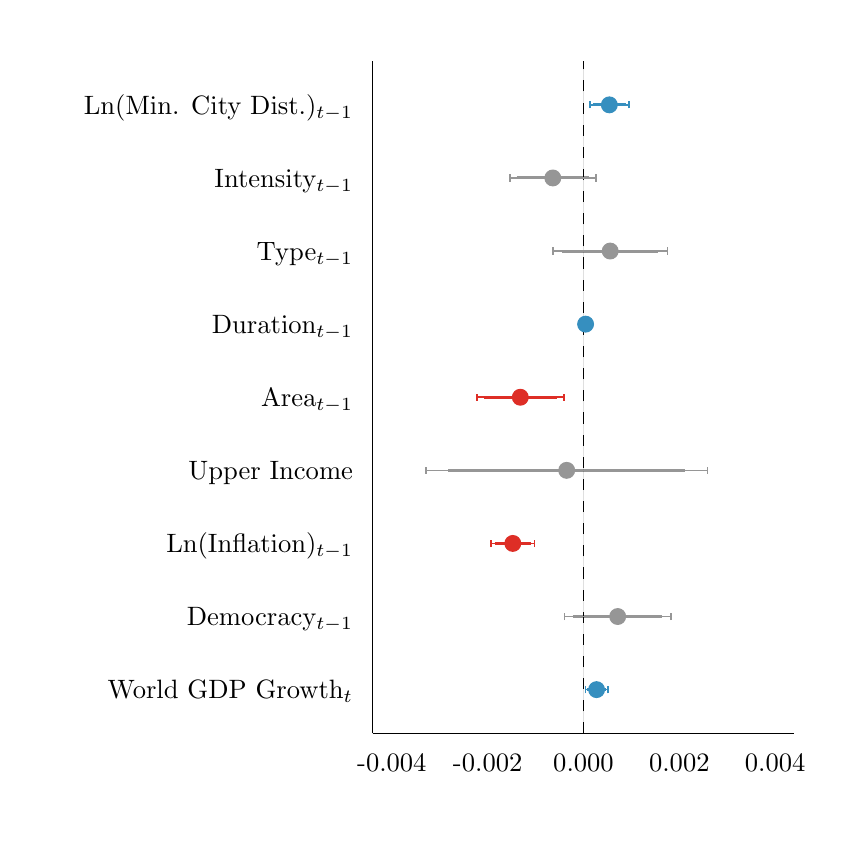
\begin{tikzpicture}[x=1pt,y=1pt]
\definecolor[named]{fillColor}{rgb}{1.00,1.00,1.00}
\path[use as bounding box,fill=fillColor,fill opacity=0.00] (0,0) rectangle (289.08,289.08);
\begin{scope}
\path[clip] (  0.00,  0.00) rectangle (289.08,289.08);
\definecolor[named]{drawColor}{rgb}{1.00,1.00,1.00}
\definecolor[named]{fillColor}{rgb}{1.00,1.00,1.00}

\path[draw=drawColor,line width= 0.6pt,line join=round,line cap=round,fill=fillColor] ( -0.00,  0.00) rectangle (289.08,289.08);
\end{scope}
\begin{scope}
\path[clip] (124.66, 34.03) rectangle (277.03,277.03);
\definecolor[named]{fillColor}{rgb}{1.00,1.00,1.00}

\path[fill=fillColor] (124.66, 34.03) rectangle (277.04,277.03);
\definecolor[named]{drawColor}{rgb}{0.21,0.56,0.75}
\definecolor[named]{fillColor}{rgb}{0.21,0.56,0.75}

\path[draw=drawColor,draw opacity=0.30,line width= 0.3pt,line join=round,fill=fillColor,fill opacity=0.30] (201.54, 49.88) -- (209.61, 49.88);
\definecolor[named]{drawColor}{rgb}{0.59,0.59,0.59}
\definecolor[named]{fillColor}{rgb}{0.59,0.59,0.59}

\path[draw=drawColor,draw opacity=0.30,line width= 0.3pt,line join=round,fill=fillColor,fill opacity=0.30] (193.96, 76.30) -- (232.45, 76.30);
\definecolor[named]{drawColor}{rgb}{0.87,0.18,0.15}
\definecolor[named]{fillColor}{rgb}{0.87,0.18,0.15}

\path[draw=drawColor,draw opacity=0.30,line width= 0.3pt,line join=round,fill=fillColor,fill opacity=0.30] (167.42,102.71) -- (183.20,102.71);
\definecolor[named]{drawColor}{rgb}{0.59,0.59,0.59}
\definecolor[named]{fillColor}{rgb}{0.59,0.59,0.59}

\path[draw=drawColor,draw opacity=0.30,line width= 0.3pt,line join=round,fill=fillColor,fill opacity=0.30] (143.88,129.12) -- (245.67,129.12);
\definecolor[named]{drawColor}{rgb}{0.87,0.18,0.15}
\definecolor[named]{fillColor}{rgb}{0.87,0.18,0.15}

\path[draw=drawColor,draw opacity=0.30,line width= 0.3pt,line join=round,fill=fillColor,fill opacity=0.30] (162.34,155.53) -- (193.68,155.53);
\definecolor[named]{drawColor}{rgb}{0.21,0.56,0.75}
\definecolor[named]{fillColor}{rgb}{0.21,0.56,0.75}

\path[draw=drawColor,draw opacity=0.30,line width= 0.3pt,line join=round,fill=fillColor,fill opacity=0.30] (200.93,181.95) -- (202.27,181.95);
\definecolor[named]{drawColor}{rgb}{0.59,0.59,0.59}
\definecolor[named]{fillColor}{rgb}{0.59,0.59,0.59}

\path[draw=drawColor,draw opacity=0.30,line width= 0.3pt,line join=round,fill=fillColor,fill opacity=0.30] (189.78,208.36) -- (231.19,208.36);

\path[draw=drawColor,draw opacity=0.30,line width= 0.3pt,line join=round,fill=fillColor,fill opacity=0.30] (174.23,234.77) -- (205.28,234.77);
\definecolor[named]{drawColor}{rgb}{0.21,0.56,0.75}
\definecolor[named]{fillColor}{rgb}{0.21,0.56,0.75}

\path[draw=drawColor,draw opacity=0.30,line width= 0.3pt,line join=round,fill=fillColor,fill opacity=0.30] (203.17,261.19) -- (217.19,261.19);
\definecolor[named]{drawColor}{rgb}{0.21,0.56,0.75}
\definecolor[named]{fillColor}{rgb}{0.21,0.56,0.75}

\path[draw=drawColor,line width= 1.1pt,line join=round,fill=fillColor] (202.19, 49.88) -- (208.96, 49.88);
\definecolor[named]{drawColor}{rgb}{0.59,0.59,0.59}
\definecolor[named]{fillColor}{rgb}{0.59,0.59,0.59}

\path[draw=drawColor,line width= 1.1pt,line join=round,fill=fillColor] (197.05, 76.30) -- (229.35, 76.30);
\definecolor[named]{drawColor}{rgb}{0.87,0.18,0.15}
\definecolor[named]{fillColor}{rgb}{0.87,0.18,0.15}

\path[draw=drawColor,line width= 1.1pt,line join=round,fill=fillColor] (168.69,102.71) -- (181.93,102.71);
\definecolor[named]{drawColor}{rgb}{0.59,0.59,0.59}
\definecolor[named]{fillColor}{rgb}{0.59,0.59,0.59}

\path[draw=drawColor,line width= 1.1pt,line join=round,fill=fillColor] (152.06,129.12) -- (237.49,129.12);
\definecolor[named]{drawColor}{rgb}{0.87,0.18,0.15}
\definecolor[named]{fillColor}{rgb}{0.87,0.18,0.15}

\path[draw=drawColor,line width= 1.1pt,line join=round,fill=fillColor] (164.86,155.53) -- (191.16,155.53);
\definecolor[named]{drawColor}{rgb}{0.21,0.56,0.75}
\definecolor[named]{fillColor}{rgb}{0.21,0.56,0.75}

\path[draw=drawColor,line width= 1.1pt,line join=round,fill=fillColor] (201.04,181.95) -- (202.16,181.95);
\definecolor[named]{drawColor}{rgb}{0.59,0.59,0.59}
\definecolor[named]{fillColor}{rgb}{0.59,0.59,0.59}

\path[draw=drawColor,line width= 1.1pt,line join=round,fill=fillColor] (193.11,208.36) -- (227.86,208.36);

\path[draw=drawColor,line width= 1.1pt,line join=round,fill=fillColor] (176.73,234.77) -- (202.79,234.77);
\definecolor[named]{drawColor}{rgb}{0.21,0.56,0.75}
\definecolor[named]{fillColor}{rgb}{0.21,0.56,0.75}

\path[draw=drawColor,line width= 1.1pt,line join=round,fill=fillColor] (204.30,261.19) -- (216.06,261.19);
\definecolor[named]{drawColor}{rgb}{0.00,0.00,0.00}
\definecolor[named]{fillColor}{rgb}{0.00,0.00,0.00}

\path[draw=drawColor,line width= 0.6pt,dash pattern=on 4pt off 4pt ,line join=round,fill=fillColor] (200.85, 34.03) -- (200.85,277.03);
\definecolor[named]{drawColor}{rgb}{0.21,0.56,0.75}
\definecolor[named]{fillColor}{rgb}{0.21,0.56,0.75}

\path[draw=drawColor,line width= 0.4pt,line join=round,line cap=round,fill=fillColor] (210.18,261.19) circle (  2.85);
\definecolor[named]{drawColor}{rgb}{0.59,0.59,0.59}
\definecolor[named]{fillColor}{rgb}{0.59,0.59,0.59}

\path[draw=drawColor,line width= 0.4pt,line join=round,line cap=round,fill=fillColor] (189.76,234.77) circle (  2.85);

\path[draw=drawColor,line width= 0.4pt,line join=round,line cap=round,fill=fillColor] (210.49,208.36) circle (  2.85);
\definecolor[named]{drawColor}{rgb}{0.21,0.56,0.75}
\definecolor[named]{fillColor}{rgb}{0.21,0.56,0.75}

\path[draw=drawColor,line width= 0.4pt,line join=round,line cap=round,fill=fillColor] (201.60,181.95) circle (  2.85);
\definecolor[named]{drawColor}{rgb}{0.87,0.18,0.15}
\definecolor[named]{fillColor}{rgb}{0.87,0.18,0.15}

\path[draw=drawColor,line width= 0.4pt,line join=round,line cap=round,fill=fillColor] (178.01,155.53) circle (  2.85);
\definecolor[named]{drawColor}{rgb}{0.59,0.59,0.59}
\definecolor[named]{fillColor}{rgb}{0.59,0.59,0.59}

\path[draw=drawColor,line width= 0.4pt,line join=round,line cap=round,fill=fillColor] (194.77,129.12) circle (  2.85);
\definecolor[named]{drawColor}{rgb}{0.87,0.18,0.15}
\definecolor[named]{fillColor}{rgb}{0.87,0.18,0.15}

\path[draw=drawColor,line width= 0.4pt,line join=round,line cap=round,fill=fillColor] (175.31,102.71) circle (  2.85);
\definecolor[named]{drawColor}{rgb}{0.59,0.59,0.59}
\definecolor[named]{fillColor}{rgb}{0.59,0.59,0.59}

\path[draw=drawColor,line width= 0.4pt,line join=round,line cap=round,fill=fillColor] (213.20, 76.30) circle (  2.85);
\definecolor[named]{drawColor}{rgb}{0.21,0.56,0.75}
\definecolor[named]{fillColor}{rgb}{0.21,0.56,0.75}

\path[draw=drawColor,line width= 0.4pt,line join=round,line cap=round,fill=fillColor] (205.57, 49.88) circle (  2.85);

\path[draw=drawColor,line width= 0.6pt,line join=round] (209.61, 48.56) --
	(209.61, 51.20);

\path[draw=drawColor,line width= 0.6pt,line join=round] (209.61, 49.88) --
	(201.54, 49.88);

\path[draw=drawColor,line width= 0.6pt,line join=round] (201.54, 48.56) --
	(201.54, 51.20);
\definecolor[named]{drawColor}{rgb}{0.59,0.59,0.59}

\path[draw=drawColor,line width= 0.6pt,line join=round] (232.45, 74.97) --
	(232.45, 77.62);

\path[draw=drawColor,line width= 0.6pt,line join=round] (232.45, 76.30) --
	(193.96, 76.30);

\path[draw=drawColor,line width= 0.6pt,line join=round] (193.96, 74.97) --
	(193.96, 77.62);
\definecolor[named]{drawColor}{rgb}{0.87,0.18,0.15}

\path[draw=drawColor,line width= 0.6pt,line join=round] (183.20,101.39) --
	(183.20,104.03);

\path[draw=drawColor,line width= 0.6pt,line join=round] (183.20,102.71) --
	(167.42,102.71);

\path[draw=drawColor,line width= 0.6pt,line join=round] (167.42,101.39) --
	(167.42,104.03);
\definecolor[named]{drawColor}{rgb}{0.59,0.59,0.59}

\path[draw=drawColor,line width= 0.6pt,line join=round] (245.67,127.80) --
	(245.67,130.44);

\path[draw=drawColor,line width= 0.6pt,line join=round] (245.67,129.12) --
	(143.88,129.12);

\path[draw=drawColor,line width= 0.6pt,line join=round] (143.88,127.80) --
	(143.88,130.44);
\definecolor[named]{drawColor}{rgb}{0.87,0.18,0.15}

\path[draw=drawColor,line width= 0.6pt,line join=round] (193.68,154.21) --
	(193.68,156.86);

\path[draw=drawColor,line width= 0.6pt,line join=round] (193.68,155.53) --
	(162.34,155.53);

\path[draw=drawColor,line width= 0.6pt,line join=round] (162.34,154.21) --
	(162.34,156.86);
\definecolor[named]{drawColor}{rgb}{0.21,0.56,0.75}

\path[draw=drawColor,line width= 0.6pt,line join=round] (202.27,180.63) --
	(202.27,183.27);

\path[draw=drawColor,line width= 0.6pt,line join=round] (202.27,181.95) --
	(200.93,181.95);

\path[draw=drawColor,line width= 0.6pt,line join=round] (200.93,180.63) --
	(200.93,183.27);
\definecolor[named]{drawColor}{rgb}{0.59,0.59,0.59}

\path[draw=drawColor,line width= 0.6pt,line join=round] (231.19,207.04) --
	(231.19,209.68);

\path[draw=drawColor,line width= 0.6pt,line join=round] (231.19,208.36) --
	(189.78,208.36);

\path[draw=drawColor,line width= 0.6pt,line join=round] (189.78,207.04) --
	(189.78,209.68);

\path[draw=drawColor,line width= 0.6pt,line join=round] (205.28,233.45) --
	(205.28,236.09);

\path[draw=drawColor,line width= 0.6pt,line join=round] (205.28,234.77) --
	(174.23,234.77);

\path[draw=drawColor,line width= 0.6pt,line join=round] (174.23,233.45) --
	(174.23,236.09);
\definecolor[named]{drawColor}{rgb}{0.21,0.56,0.75}

\path[draw=drawColor,line width= 0.6pt,line join=round] (217.19,259.87) --
	(217.19,262.51);

\path[draw=drawColor,line width= 0.6pt,line join=round] (217.19,261.19) --
	(203.17,261.19);

\path[draw=drawColor,line width= 0.6pt,line join=round] (203.17,259.87) --
	(203.17,262.51);
\end{scope}
\begin{scope}
\path[clip] (  0.00,  0.00) rectangle (289.08,289.08);
\definecolor[named]{drawColor}{rgb}{0.00,0.00,0.00}

\path[draw=drawColor,line width= 0.6pt,line join=round] (124.66, 34.03) --
	(124.66,277.03);
\end{scope}
\begin{scope}
\path[clip] (  0.00,  0.00) rectangle (289.08,289.08);
\definecolor[named]{drawColor}{rgb}{0.00,0.00,0.00}

\node[text=drawColor,anchor=base east,inner sep=0pt, outer sep=0pt, scale=  0.96] at (117.55, 46.58) {World GDP Growth$_{t}$};

\node[text=drawColor,anchor=base east,inner sep=0pt, outer sep=0pt, scale=  0.96] at (117.55, 72.99) {Democracy$_{t-1}$};

\node[text=drawColor,anchor=base east,inner sep=0pt, outer sep=0pt, scale=  0.96] at (117.55, 99.40) {Ln(Inflation)$_{t-1}$};

\node[text=drawColor,anchor=base east,inner sep=0pt, outer sep=0pt, scale=  0.96] at (117.55,125.82) {Upper Income};

\node[text=drawColor,anchor=base east,inner sep=0pt, outer sep=0pt, scale=  0.96] at (117.55,152.23) {Area$_{t-1}$};

\node[text=drawColor,anchor=base east,inner sep=0pt, outer sep=0pt, scale=  0.96] at (117.55,178.64) {Duration$_{t-1}$};

\node[text=drawColor,anchor=base east,inner sep=0pt, outer sep=0pt, scale=  0.96] at (117.55,205.06) {Type$_{t-1}$};

\node[text=drawColor,anchor=base east,inner sep=0pt, outer sep=0pt, scale=  0.96] at (117.55,231.47) {Intensity$_{t-1}$};

\node[text=drawColor,anchor=base east,inner sep=0pt, outer sep=0pt, scale=  0.96] at (117.55,257.88) {Ln(Min. City Dist.)$_{t-1}$};
\end{scope}
\begin{scope}
\path[clip] (  0.00,  0.00) rectangle (289.08,289.08);
\definecolor[named]{drawColor}{rgb}{0.00,0.00,0.00}

\path[draw=drawColor,line width= 0.6pt,line join=round] (124.66, 34.03) --
	(277.03, 34.03);
\end{scope}
\begin{scope}
\path[clip] (  0.00,  0.00) rectangle (289.08,289.08);
\definecolor[named]{drawColor}{rgb}{0.00,0.00,0.00}

\node[text=drawColor,anchor=base,inner sep=0pt, outer sep=0pt, scale=  0.96] at (131.59, 20.31) {-0.004};

\node[text=drawColor,anchor=base,inner sep=0pt, outer sep=0pt, scale=  0.96] at (166.22, 20.31) {-0.002};

\node[text=drawColor,anchor=base,inner sep=0pt, outer sep=0pt, scale=  0.96] at (200.85, 20.31) {0.000};

\node[text=drawColor,anchor=base,inner sep=0pt, outer sep=0pt, scale=  0.96] at (235.48, 20.31) {0.002};

\node[text=drawColor,anchor=base,inner sep=0pt, outer sep=0pt, scale=  0.96] at (270.11, 20.31) {0.004};
\end{scope}
\end{tikzpicture}
}
	\end{tabular}
\end{figure}

\end{frame}
%%%%%%%%%%%%%%%%%%%%%%%%%%%%%%%%%%%%%%%%%

%%%%%%%%%%%%%%%%%%%%%%%%%%%%%%%%%%%%%%%%%
\begin{frame}
\frametitle{Cross-Validation of Parameter Estimates}

\begin{figure}[ht]
	\centering
	\resizebox{1\textwidth}{!}{% Created by tikzDevice version 0.7.0 on 2014-10-06 19:49:11
% !TEX encoding = UTF-8 Unicode
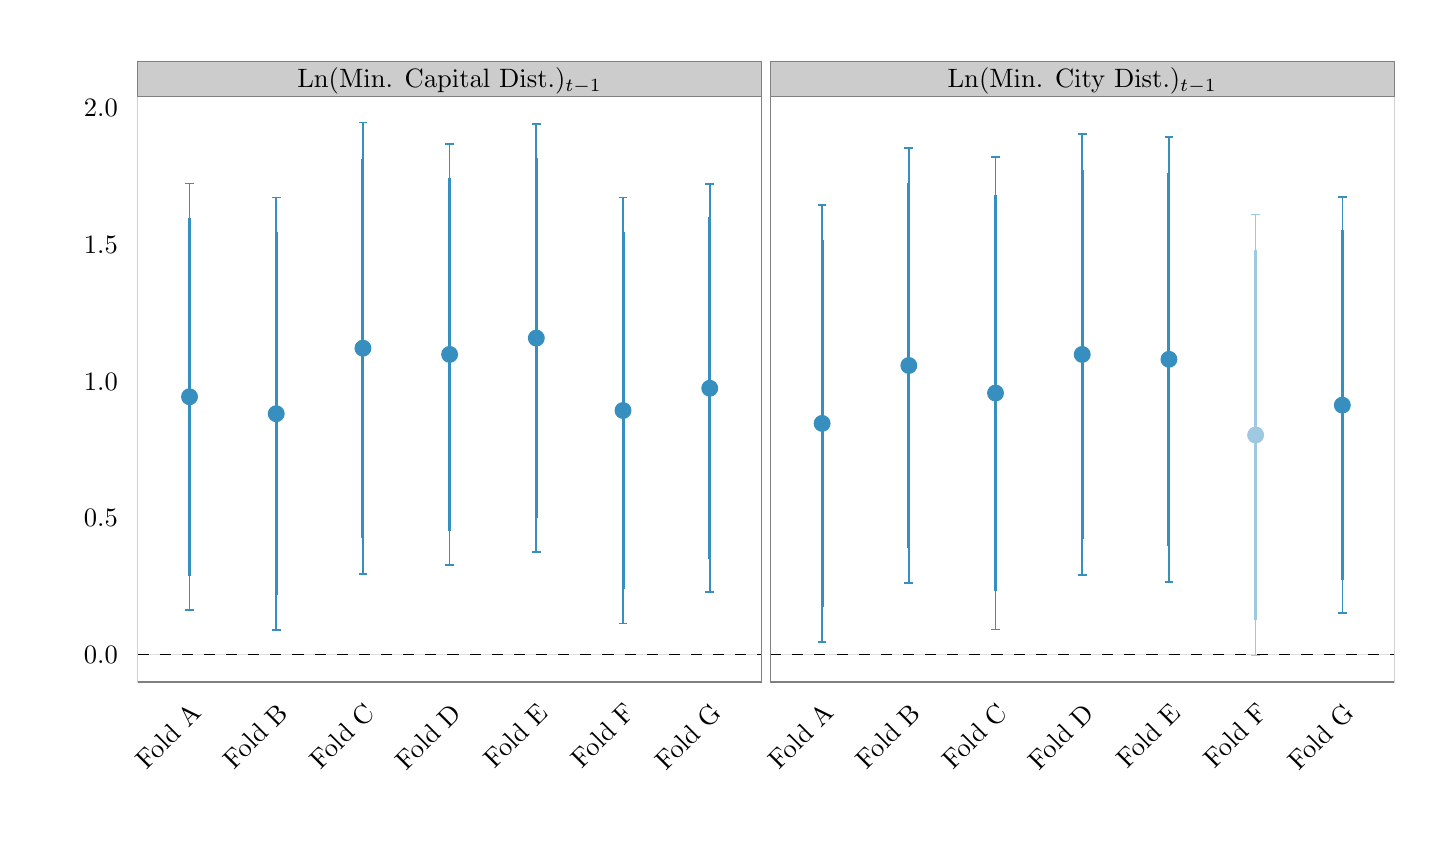
\begin{tikzpicture}[x=1pt,y=1pt]
\definecolor[named]{fillColor}{rgb}{1.00,1.00,1.00}
\path[use as bounding box,fill=fillColor,fill opacity=0.00] (0,0) rectangle (505.89,289.08);
\begin{scope}
\path[clip] (  0.00,  0.00) rectangle (505.89,289.08);
\definecolor[named]{drawColor}{rgb}{1.00,1.00,1.00}
\definecolor[named]{fillColor}{rgb}{1.00,1.00,1.00}

\path[draw=drawColor,line width= 0.6pt,line join=round,line cap=round,fill=fillColor] (  0.00,  0.00) rectangle (505.89,289.08);
\end{scope}
\begin{scope}
\path[clip] ( 39.69, 52.60) rectangle (265.26,264.40);
\definecolor[named]{fillColor}{rgb}{1.00,1.00,1.00}

\path[fill=fillColor] ( 39.69, 52.60) rectangle (265.26,264.40);
\definecolor[named]{drawColor}{rgb}{0.21,0.56,0.75}
\definecolor[named]{fillColor}{rgb}{0.21,0.56,0.75}

\path[draw=drawColor,draw opacity=0.30,line width= 0.3pt,line join=round,fill=fillColor,fill opacity=0.30] ( 58.48, 78.70) -- ( 58.48,232.72);

\path[draw=drawColor,draw opacity=0.30,line width= 0.3pt,line join=round,fill=fillColor,fill opacity=0.30] ( 89.81, 71.45) -- ( 89.81,227.72);

\path[draw=drawColor,draw opacity=0.30,line width= 0.3pt,line join=round,fill=fillColor,fill opacity=0.30] (121.14, 91.74) -- (121.14,254.77);

\path[draw=drawColor,draw opacity=0.30,line width= 0.3pt,line join=round,fill=fillColor,fill opacity=0.30] (152.47, 95.01) -- (152.47,247.01);

\path[draw=drawColor,draw opacity=0.30,line width= 0.3pt,line join=round,fill=fillColor,fill opacity=0.30] (183.80, 99.56) -- (183.80,254.25);

\path[draw=drawColor,draw opacity=0.30,line width= 0.3pt,line join=round,fill=fillColor,fill opacity=0.30] (215.13, 73.72) -- (215.13,227.75);

\path[draw=drawColor,draw opacity=0.30,line width= 0.3pt,line join=round,fill=fillColor,fill opacity=0.30] (246.46, 85.07) -- (246.46,232.49);
\definecolor[named]{drawColor}{rgb}{0.21,0.56,0.75}
\definecolor[named]{fillColor}{rgb}{0.21,0.56,0.75}

\path[draw=drawColor,line width= 1.1pt,line join=round,fill=fillColor] ( 58.48, 91.09) -- ( 58.48,220.34);

\path[draw=drawColor,line width= 1.1pt,line join=round,fill=fillColor] ( 89.81, 84.01) -- ( 89.81,215.15);

\path[draw=drawColor,line width= 1.1pt,line join=round,fill=fillColor] (121.14,104.85) -- (121.14,241.67);

\path[draw=drawColor,line width= 1.1pt,line join=round,fill=fillColor] (152.47,107.23) -- (152.47,234.79);

\path[draw=drawColor,line width= 1.1pt,line join=round,fill=fillColor] (183.80,111.99) -- (183.80,241.82);

\path[draw=drawColor,line width= 1.1pt,line join=round,fill=fillColor] (215.13, 86.11) -- (215.13,215.37);

\path[draw=drawColor,line width= 1.1pt,line join=round,fill=fillColor] (246.46, 96.92) -- (246.46,220.64);
\definecolor[named]{drawColor}{rgb}{0.00,0.00,0.00}
\definecolor[named]{fillColor}{rgb}{0.00,0.00,0.00}

\path[draw=drawColor,line width= 0.6pt,dash pattern=on 4pt off 4pt ,line join=round,fill=fillColor] ( 39.69, 62.52) -- (265.26, 62.52);
\definecolor[named]{drawColor}{rgb}{0.21,0.56,0.75}
\definecolor[named]{fillColor}{rgb}{0.21,0.56,0.75}

\path[draw=drawColor,line width= 0.4pt,line join=round,line cap=round,fill=fillColor] ( 58.48,155.71) circle (  2.85);

\path[draw=drawColor,line width= 0.4pt,line join=round,line cap=round,fill=fillColor] ( 89.81,149.58) circle (  2.85);

\path[draw=drawColor,line width= 0.4pt,line join=round,line cap=round,fill=fillColor] (121.14,173.26) circle (  2.85);

\path[draw=drawColor,line width= 0.4pt,line join=round,line cap=round,fill=fillColor] (152.47,171.01) circle (  2.85);

\path[draw=drawColor,line width= 0.4pt,line join=round,line cap=round,fill=fillColor] (183.80,176.91) circle (  2.85);

\path[draw=drawColor,line width= 0.4pt,line join=round,line cap=round,fill=fillColor] (215.13,150.74) circle (  2.85);

\path[draw=drawColor,line width= 0.4pt,line join=round,line cap=round,fill=fillColor] (246.46,158.78) circle (  2.85);

\path[draw=drawColor,line width= 0.6pt,line join=round] ( 56.92,232.72) --
	( 60.05,232.72);

\path[draw=drawColor,line width= 0.6pt,line join=round] ( 58.48,232.72) --
	( 58.48, 78.70);

\path[draw=drawColor,line width= 0.6pt,line join=round] ( 56.92, 78.70) --
	( 60.05, 78.70);

\path[draw=drawColor,line width= 0.6pt,line join=round] ( 88.25,227.72) --
	( 91.38,227.72);

\path[draw=drawColor,line width= 0.6pt,line join=round] ( 89.81,227.72) --
	( 89.81, 71.45);

\path[draw=drawColor,line width= 0.6pt,line join=round] ( 88.25, 71.45) --
	( 91.38, 71.45);

\path[draw=drawColor,line width= 0.6pt,line join=round] (119.58,254.77) --
	(122.71,254.77);

\path[draw=drawColor,line width= 0.6pt,line join=round] (121.14,254.77) --
	(121.14, 91.74);

\path[draw=drawColor,line width= 0.6pt,line join=round] (119.58, 91.74) --
	(122.71, 91.74);

\path[draw=drawColor,line width= 0.6pt,line join=round] (150.91,247.01) --
	(154.04,247.01);

\path[draw=drawColor,line width= 0.6pt,line join=round] (152.47,247.01) --
	(152.47, 95.01);

\path[draw=drawColor,line width= 0.6pt,line join=round] (150.91, 95.01) --
	(154.04, 95.01);

\path[draw=drawColor,line width= 0.6pt,line join=round] (182.24,254.25) --
	(185.37,254.25);

\path[draw=drawColor,line width= 0.6pt,line join=round] (183.80,254.25) --
	(183.80, 99.56);

\path[draw=drawColor,line width= 0.6pt,line join=round] (182.24, 99.56) --
	(185.37, 99.56);

\path[draw=drawColor,line width= 0.6pt,line join=round] (213.57,227.75) --
	(216.70,227.75);

\path[draw=drawColor,line width= 0.6pt,line join=round] (215.13,227.75) --
	(215.13, 73.72);

\path[draw=drawColor,line width= 0.6pt,line join=round] (213.57, 73.72) --
	(216.70, 73.72);

\path[draw=drawColor,line width= 0.6pt,line join=round] (244.90,232.49) --
	(248.03,232.49);

\path[draw=drawColor,line width= 0.6pt,line join=round] (246.46,232.49) --
	(246.46, 85.07);

\path[draw=drawColor,line width= 0.6pt,line join=round] (244.90, 85.07) --
	(248.03, 85.07);
\definecolor[named]{drawColor}{rgb}{0.50,0.50,0.50}

\path[draw=drawColor,line width= 0.6pt,line join=round,line cap=round] ( 39.69, 52.60) rectangle (265.26,264.40);
\end{scope}
\begin{scope}
\path[clip] (268.27, 52.60) rectangle (493.85,264.40);
\definecolor[named]{fillColor}{rgb}{1.00,1.00,1.00}

\path[fill=fillColor] (268.27, 52.60) rectangle (493.85,264.40);
\definecolor[named]{drawColor}{rgb}{0.21,0.56,0.75}
\definecolor[named]{fillColor}{rgb}{0.21,0.56,0.75}

\path[draw=drawColor,draw opacity=0.30,line width= 0.3pt,line join=round,fill=fillColor,fill opacity=0.30] (287.07, 67.19) -- (287.07,224.97);

\path[draw=drawColor,draw opacity=0.30,line width= 0.3pt,line join=round,fill=fillColor,fill opacity=0.30] (318.40, 88.38) -- (318.40,245.63);

\path[draw=drawColor,draw opacity=0.30,line width= 0.3pt,line join=round,fill=fillColor,fill opacity=0.30] (349.73, 71.61) -- (349.73,242.46);

\path[draw=drawColor,draw opacity=0.30,line width= 0.3pt,line join=round,fill=fillColor,fill opacity=0.30] (381.06, 91.40) -- (381.06,250.60);

\path[draw=drawColor,draw opacity=0.30,line width= 0.3pt,line join=round,fill=fillColor,fill opacity=0.30] (412.39, 88.88) -- (412.39,249.59);
\definecolor[named]{drawColor}{rgb}{0.62,0.79,0.88}
\definecolor[named]{fillColor}{rgb}{0.62,0.79,0.88}

\path[draw=drawColor,draw opacity=0.30,line width= 0.3pt,line join=round,fill=fillColor,fill opacity=0.30] (443.72, 62.23) -- (443.72,221.53);
\definecolor[named]{drawColor}{rgb}{0.21,0.56,0.75}
\definecolor[named]{fillColor}{rgb}{0.21,0.56,0.75}

\path[draw=drawColor,draw opacity=0.30,line width= 0.3pt,line join=round,fill=fillColor,fill opacity=0.30] (475.05, 77.47) -- (475.05,227.88);
\definecolor[named]{drawColor}{rgb}{0.21,0.56,0.75}
\definecolor[named]{fillColor}{rgb}{0.21,0.56,0.75}

\path[draw=drawColor,line width= 1.1pt,line join=round,fill=fillColor] (287.07, 79.88) -- (287.07,212.29);

\path[draw=drawColor,line width= 1.1pt,line join=round,fill=fillColor] (318.40,101.02) -- (318.40,232.99);

\path[draw=drawColor,line width= 1.1pt,line join=round,fill=fillColor] (349.73, 85.35) -- (349.73,228.72);

\path[draw=drawColor,line width= 1.1pt,line join=round,fill=fillColor] (381.06,104.20) -- (381.06,237.81);

\path[draw=drawColor,line width= 1.1pt,line join=round,fill=fillColor] (412.39,101.80) -- (412.39,236.67);
\definecolor[named]{drawColor}{rgb}{0.62,0.79,0.88}
\definecolor[named]{fillColor}{rgb}{0.62,0.79,0.88}

\path[draw=drawColor,line width= 1.1pt,line join=round,fill=fillColor] (443.72, 75.03) -- (443.72,208.73);
\definecolor[named]{drawColor}{rgb}{0.21,0.56,0.75}
\definecolor[named]{fillColor}{rgb}{0.21,0.56,0.75}

\path[draw=drawColor,line width= 1.1pt,line join=round,fill=fillColor] (475.05, 89.56) -- (475.05,215.79);
\definecolor[named]{drawColor}{rgb}{0.00,0.00,0.00}
\definecolor[named]{fillColor}{rgb}{0.00,0.00,0.00}

\path[draw=drawColor,line width= 0.6pt,dash pattern=on 4pt off 4pt ,line join=round,fill=fillColor] (268.27, 62.52) -- (493.85, 62.52);
\definecolor[named]{drawColor}{rgb}{0.21,0.56,0.75}
\definecolor[named]{fillColor}{rgb}{0.21,0.56,0.75}

\path[draw=drawColor,line width= 0.4pt,line join=round,line cap=round,fill=fillColor] (287.07,146.08) circle (  2.85);

\path[draw=drawColor,line width= 0.4pt,line join=round,line cap=round,fill=fillColor] (318.40,167.00) circle (  2.85);

\path[draw=drawColor,line width= 0.4pt,line join=round,line cap=round,fill=fillColor] (349.73,157.04) circle (  2.85);

\path[draw=drawColor,line width= 0.4pt,line join=round,line cap=round,fill=fillColor] (381.06,171.00) circle (  2.85);

\path[draw=drawColor,line width= 0.4pt,line join=round,line cap=round,fill=fillColor] (412.39,169.24) circle (  2.85);
\definecolor[named]{drawColor}{rgb}{0.62,0.79,0.88}
\definecolor[named]{fillColor}{rgb}{0.62,0.79,0.88}

\path[draw=drawColor,line width= 0.4pt,line join=round,line cap=round,fill=fillColor] (443.72,141.88) circle (  2.85);
\definecolor[named]{drawColor}{rgb}{0.21,0.56,0.75}
\definecolor[named]{fillColor}{rgb}{0.21,0.56,0.75}

\path[draw=drawColor,line width= 0.4pt,line join=round,line cap=round,fill=fillColor] (475.05,152.67) circle (  2.85);

\path[draw=drawColor,line width= 0.6pt,line join=round] (285.50,224.97) --
	(288.64,224.97);

\path[draw=drawColor,line width= 0.6pt,line join=round] (287.07,224.97) --
	(287.07, 67.19);

\path[draw=drawColor,line width= 0.6pt,line join=round] (285.50, 67.19) --
	(288.64, 67.19);

\path[draw=drawColor,line width= 0.6pt,line join=round] (316.83,245.63) --
	(319.97,245.63);

\path[draw=drawColor,line width= 0.6pt,line join=round] (318.40,245.63) --
	(318.40, 88.38);

\path[draw=drawColor,line width= 0.6pt,line join=round] (316.83, 88.38) --
	(319.97, 88.38);

\path[draw=drawColor,line width= 0.6pt,line join=round] (348.16,242.46) --
	(351.30,242.46);

\path[draw=drawColor,line width= 0.6pt,line join=round] (349.73,242.46) --
	(349.73, 71.61);

\path[draw=drawColor,line width= 0.6pt,line join=round] (348.16, 71.61) --
	(351.30, 71.61);

\path[draw=drawColor,line width= 0.6pt,line join=round] (379.49,250.60) --
	(382.62,250.60);

\path[draw=drawColor,line width= 0.6pt,line join=round] (381.06,250.60) --
	(381.06, 91.40);

\path[draw=drawColor,line width= 0.6pt,line join=round] (379.49, 91.40) --
	(382.62, 91.40);

\path[draw=drawColor,line width= 0.6pt,line join=round] (410.82,249.59) --
	(413.95,249.59);

\path[draw=drawColor,line width= 0.6pt,line join=round] (412.39,249.59) --
	(412.39, 88.88);

\path[draw=drawColor,line width= 0.6pt,line join=round] (410.82, 88.88) --
	(413.95, 88.88);
\definecolor[named]{drawColor}{rgb}{0.62,0.79,0.88}

\path[draw=drawColor,line width= 0.6pt,line join=round] (442.15,221.53) --
	(445.28,221.53);

\path[draw=drawColor,line width= 0.6pt,line join=round] (443.72,221.53) --
	(443.72, 62.23);

\path[draw=drawColor,line width= 0.6pt,line join=round] (442.15, 62.23) --
	(445.28, 62.23);
\definecolor[named]{drawColor}{rgb}{0.21,0.56,0.75}

\path[draw=drawColor,line width= 0.6pt,line join=round] (473.48,227.88) --
	(476.61,227.88);

\path[draw=drawColor,line width= 0.6pt,line join=round] (475.05,227.88) --
	(475.05, 77.47);

\path[draw=drawColor,line width= 0.6pt,line join=round] (473.48, 77.47) --
	(476.61, 77.47);
\definecolor[named]{drawColor}{rgb}{0.50,0.50,0.50}

\path[draw=drawColor,line width= 0.6pt,line join=round,line cap=round] (268.27, 52.60) rectangle (493.85,264.40);
\end{scope}
\begin{scope}
\path[clip] (  0.00,  0.00) rectangle (505.89,289.08);
\definecolor[named]{drawColor}{rgb}{0.50,0.50,0.50}
\definecolor[named]{fillColor}{rgb}{0.80,0.80,0.80}

\path[draw=drawColor,line width= 0.2pt,line join=round,line cap=round,fill=fillColor] ( 39.69,264.40) rectangle (265.26,277.04);
\definecolor[named]{drawColor}{rgb}{0.00,0.00,0.00}

\node[text=drawColor,anchor=base,inner sep=0pt, outer sep=0pt, scale=  0.96] at (152.47,267.41) {Ln(Min. Capital Dist.)$_{t-1}$};
\end{scope}
\begin{scope}
\path[clip] (  0.00,  0.00) rectangle (505.89,289.08);
\definecolor[named]{drawColor}{rgb}{0.50,0.50,0.50}
\definecolor[named]{fillColor}{rgb}{0.80,0.80,0.80}

\path[draw=drawColor,line width= 0.2pt,line join=round,line cap=round,fill=fillColor] (268.27,264.40) rectangle (493.85,277.04);
\definecolor[named]{drawColor}{rgb}{0.00,0.00,0.00}

\node[text=drawColor,anchor=base,inner sep=0pt, outer sep=0pt, scale=  0.96] at (381.06,267.41) {Ln(Min. City Dist.)$_{t-1}$};
\end{scope}
\begin{scope}
\path[clip] (  0.00,  0.00) rectangle (505.89,289.08);
\definecolor[named]{drawColor}{rgb}{0.00,0.00,0.00}

\node[text=drawColor,anchor=base east,inner sep=0pt, outer sep=0pt, scale=  0.96] at ( 32.57, 59.21) {0.0};

\node[text=drawColor,anchor=base east,inner sep=0pt, outer sep=0pt, scale=  0.96] at ( 32.57,108.66) {0.5};

\node[text=drawColor,anchor=base east,inner sep=0pt, outer sep=0pt, scale=  0.96] at ( 32.57,158.12) {1.0};

\node[text=drawColor,anchor=base east,inner sep=0pt, outer sep=0pt, scale=  0.96] at ( 32.57,207.57) {1.5};

\node[text=drawColor,anchor=base east,inner sep=0pt, outer sep=0pt, scale=  0.96] at ( 32.57,257.02) {2.0};
\end{scope}
\begin{scope}
\path[clip] (  0.00,  0.00) rectangle (505.89,289.08);
\definecolor[named]{drawColor}{rgb}{0.00,0.00,0.00}

\node[text=drawColor,rotate= 45.00,anchor=base east,inner sep=0pt, outer sep=0pt, scale=  0.96] at ( 63.16, 40.81) {Fold A};

\node[text=drawColor,rotate= 45.00,anchor=base east,inner sep=0pt, outer sep=0pt, scale=  0.96] at ( 94.49, 40.81) {Fold B};

\node[text=drawColor,rotate= 45.00,anchor=base east,inner sep=0pt, outer sep=0pt, scale=  0.96] at (125.82, 40.81) {Fold C};

\node[text=drawColor,rotate= 45.00,anchor=base east,inner sep=0pt, outer sep=0pt, scale=  0.96] at (157.15, 40.81) {Fold D};

\node[text=drawColor,rotate= 45.00,anchor=base east,inner sep=0pt, outer sep=0pt, scale=  0.96] at (188.48, 40.81) {Fold E};

\node[text=drawColor,rotate= 45.00,anchor=base east,inner sep=0pt, outer sep=0pt, scale=  0.96] at (219.81, 40.81) {Fold F};

\node[text=drawColor,rotate= 45.00,anchor=base east,inner sep=0pt, outer sep=0pt, scale=  0.96] at (251.14, 40.81) {Fold G};
\end{scope}
\begin{scope}
\path[clip] (  0.00,  0.00) rectangle (505.89,289.08);
\definecolor[named]{drawColor}{rgb}{0.00,0.00,0.00}

\node[text=drawColor,rotate= 45.00,anchor=base east,inner sep=0pt, outer sep=0pt, scale=  0.96] at (291.74, 40.81) {Fold A};

\node[text=drawColor,rotate= 45.00,anchor=base east,inner sep=0pt, outer sep=0pt, scale=  0.96] at (323.07, 40.81) {Fold B};

\node[text=drawColor,rotate= 45.00,anchor=base east,inner sep=0pt, outer sep=0pt, scale=  0.96] at (354.40, 40.81) {Fold C};

\node[text=drawColor,rotate= 45.00,anchor=base east,inner sep=0pt, outer sep=0pt, scale=  0.96] at (385.73, 40.81) {Fold D};

\node[text=drawColor,rotate= 45.00,anchor=base east,inner sep=0pt, outer sep=0pt, scale=  0.96] at (417.06, 40.81) {Fold E};

\node[text=drawColor,rotate= 45.00,anchor=base east,inner sep=0pt, outer sep=0pt, scale=  0.96] at (448.39, 40.81) {Fold F};

\node[text=drawColor,rotate= 45.00,anchor=base east,inner sep=0pt, outer sep=0pt, scale=  0.96] at (479.72, 40.81) {Fold G};
\end{scope}
\end{tikzpicture}
}
\end{figure}

\end{frame}
%%%%%%%%%%%%%%%%%%%%%%%%%%%%%%%%%%%%%%%%%

%%%%%%%%%%%%%%%%%%%%%%%%%%%%%%%%%%%%%%%%%
\begin{frame}
\frametitle{Substantive Effects: Capital Distance}

\vspace{-6mm}
\begin{figure}
	\centering
	\resizebox{1\textwidth}{!}{% Created by tikzDevice version 0.7.0 on 2014-10-06 19:44:45
% !TEX encoding = UTF-8 Unicode
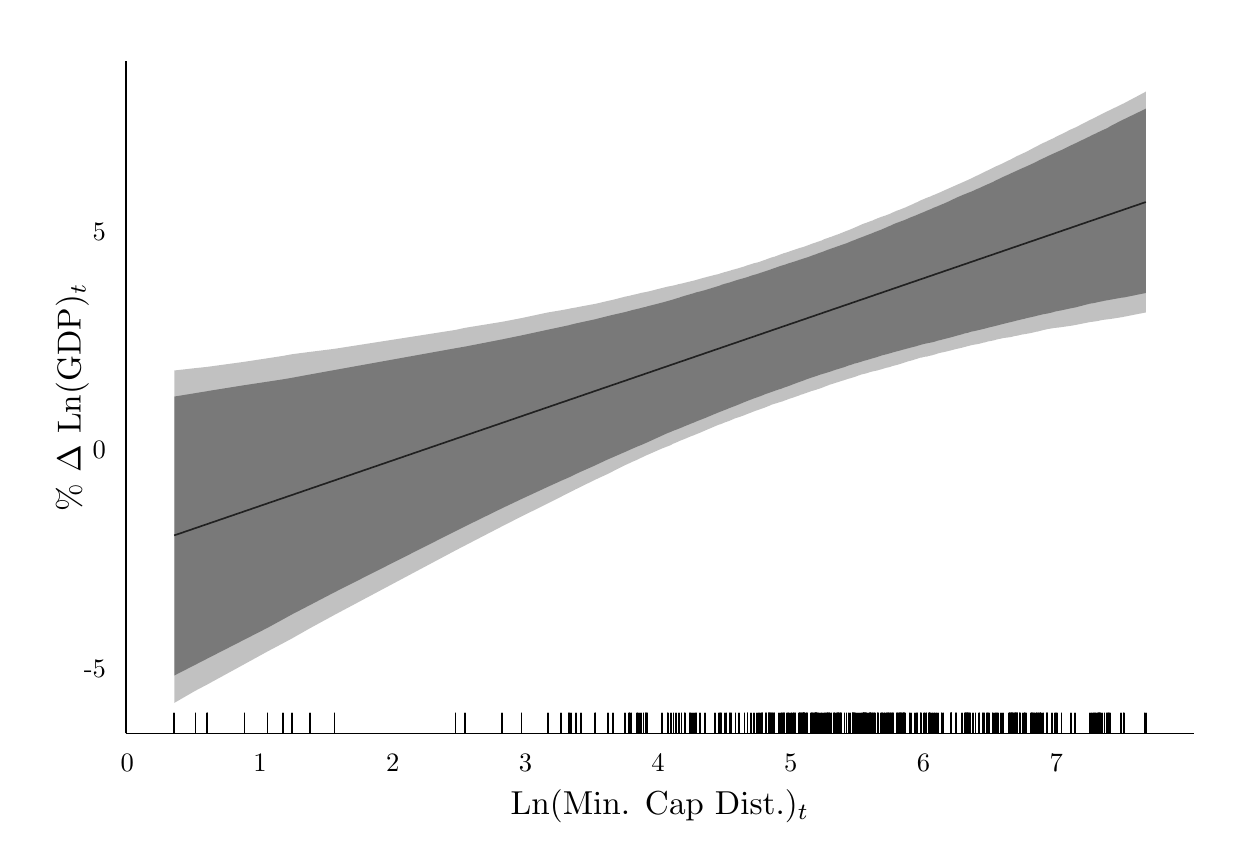
\begin{tikzpicture}[x=1pt,y=1pt]
\definecolor[named]{fillColor}{rgb}{1.00,1.00,1.00}
\path[use as bounding box,fill=fillColor,fill opacity=0.00] (0,0) rectangle (433.62,289.08);
\begin{scope}
\path[clip] (  0.00,  0.00) rectangle (433.62,289.08);
\definecolor[named]{drawColor}{rgb}{1.00,1.00,1.00}
\definecolor[named]{fillColor}{rgb}{1.00,1.00,1.00}

\path[draw=drawColor,line width= 0.6pt,line join=round,line cap=round,fill=fillColor] (  0.00,  0.00) rectangle (433.62,289.08);
\end{scope}
\begin{scope}
\path[clip] ( 35.42, 34.03) rectangle (421.57,277.03);
\definecolor[named]{fillColor}{rgb}{1.00,1.00,1.00}

\path[fill=fillColor] ( 35.42, 34.03) rectangle (421.57,277.03);
\definecolor[named]{drawColor}{rgb}{0.00,0.00,0.00}

\path[draw=drawColor,line width= 0.6pt,line join=round] ( 52.97,105.62) --
	( 60.61,108.24) --
	( 64.85,109.70) --
	( 64.98,109.74) --
	( 78.30,114.31) --
	( 86.71,117.20) --
	( 92.34,119.13) --
	( 95.59,120.24) --
	(101.92,122.42) --
	(110.88,125.49) --
	(154.64,140.51) --
	(158.01,141.66) --
	(171.43,146.26) --
	(178.49,148.69) --
	(187.92,151.92) --
	(192.71,153.57) --
	(195.62,154.56) --
	(195.71,154.59) --
	(196.35,154.81) --
	(198.04,155.39) --
	(199.87,156.02) --
	(204.99,157.78) --
	(205.19,157.85) --
	(209.65,159.38) --
	(211.50,160.01) --
	(215.87,161.51) --
	(217.33,162.01) --
	(217.43,162.05) --
	(217.68,162.13) --
	(218.17,162.30) --
	(220.17,162.99) --
	(220.33,163.04) --
	(220.93,163.25) --
	(221.63,163.49) --
	(222.58,163.81) --
	(223.29,164.06) --
	(223.54,164.14) --
	(223.59,164.16) --
	(224.00,164.30) --
	(229.14,166.07) --
	(231.15,166.76) --
	(231.34,166.82) --
	(232.39,167.18) --
	(233.34,167.51) --
	(234.25,167.82) --
	(235.24,168.16) --
	(236.22,168.49) --
	(237.40,168.90) --
	(237.41,168.90) --
	(239.29,169.55) --
	(239.31,169.55) --
	(240.03,169.80) --
	(240.80,170.06) --
	(241.27,170.23) --
	(241.65,170.36) --
	(242.95,170.80) --
	(244.78,171.43) --
	(248.30,172.64) --
	(249.74,173.13) --
	(250.22,173.30) --
	(250.38,173.35) --
	(250.69,173.46) --
	(251.97,173.90) --
	(252.46,174.07) --
	(253.69,174.49) --
	(253.89,174.55) --
	(254.34,174.71) --
	(255.74,175.19) --
	(256.94,175.60) --
	(258.99,176.31) --
	(260.08,176.68) --
	(260.16,176.71) --
	(261.39,177.13) --
	(262.57,177.53) --
	(263.47,177.84) --
	(264.14,178.07) --
	(264.43,178.17) --
	(264.94,178.35) --
	(265.11,178.40) --
	(265.48,178.53) --
	(265.54,178.55) --
	(266.69,178.95) --
	(266.70,178.95) --
	(267.74,179.31) --
	(267.83,179.34) --
	(267.95,179.38) --
	(268.15,179.45) --
	(268.32,179.51) --
	(268.51,179.57) --
	(268.75,179.66) --
	(269.12,179.78) --
	(269.30,179.84) --
	(269.75,180.00) --
	(269.91,180.05) --
	(271.51,180.60) --
	(272.31,180.88) --
	(272.40,180.91) --
	(272.91,181.08) --
	(273.01,181.11) --
	(273.29,181.21) --
	(273.48,181.28) --
	(274.31,181.56) --
	(274.85,181.75) --
	(274.88,181.76) --
	(275.50,181.97) --
	(276.03,182.15) --
	(276.14,182.19) --
	(276.73,182.39) --
	(276.77,182.41) --
	(277.28,182.58) --
	(277.37,182.61) --
	(278.83,183.11) --
	(278.93,183.15) --
	(278.99,183.17) --
	(279.03,183.18) --
	(279.36,183.30) --
	(279.83,183.46) --
	(279.90,183.48) --
	(280.21,183.59) --
	(280.36,183.64) --
	(280.41,183.66) --
	(280.47,183.68) --
	(280.50,183.68) --
	(280.60,183.72) --
	(280.63,183.73) --
	(281.16,183.91) --
	(281.52,184.03) --
	(281.60,184.06) --
	(283.10,184.58) --
	(283.28,184.64) --
	(283.34,184.66) --
	(283.74,184.80) --
	(283.80,184.82) --
	(284.26,184.97) --
	(284.43,185.03) --
	(284.75,185.14) --
	(284.80,185.16) --
	(284.81,185.16) --
	(284.81,185.16) --
	(284.84,185.18) --
	(284.88,185.19) --
	(285.44,185.38) --
	(285.67,185.46) --
	(286.04,185.59) --
	(286.70,185.81) --
	(286.95,185.90) --
	(287.76,186.18) --
	(288.16,186.31) --
	(288.45,186.41) --
	(288.86,186.55) --
	(289.03,186.61) --
	(289.13,186.65) --
	(289.30,186.70) --
	(289.61,186.81) --
	(289.71,186.85) --
	(289.99,186.94) --
	(290.44,187.10) --
	(291.29,187.39) --
	(291.45,187.44) --
	(291.58,187.49) --
	(292.20,187.70) --
	(292.36,187.75) --
	(292.77,187.89) --
	(292.78,187.90) --
	(292.85,187.92) --
	(292.94,187.95) --
	(293.49,188.14) --
	(293.61,188.18) --
	(293.90,188.28) --
	(293.94,188.30) --
	(295.12,188.70) --
	(295.85,188.95) --
	(296.61,189.21) --
	(297.11,189.38) --
	(297.99,189.68) --
	(298.09,189.72) --
	(298.13,189.74) --
	(298.21,189.76) --
	(298.45,189.84) --
	(298.48,189.85) --
	(298.71,189.93) --
	(298.89,190.00) --
	(299.22,190.11) --
	(300.07,190.40) --
	(300.69,190.61) --
	(301.34,190.83) --
	(301.81,191.00) --
	(301.86,191.01) --
	(302.06,191.08) --
	(302.08,191.09) --
	(302.20,191.13) --
	(302.30,191.16) --
	(302.45,191.22) --
	(302.52,191.24) --
	(302.61,191.27) --
	(302.89,191.37) --
	(302.93,191.38) --
	(303.17,191.46) --
	(304.10,191.78) --
	(304.31,191.85) --
	(304.47,191.91) --
	(304.48,191.91) --
	(304.60,191.95) --
	(304.68,191.98) --
	(305.11,192.13) --
	(305.28,192.19) --
	(305.76,192.35) --
	(305.86,192.39) --
	(306.15,192.49) --
	(307.03,192.79) --
	(307.16,192.83) --
	(307.37,192.90) --
	(308.42,193.27) --
	(308.63,193.34) --
	(308.79,193.39) --
	(309.08,193.49) --
	(309.55,193.65) --
	(309.72,193.71) --
	(310.36,193.93) --
	(310.45,193.96) --
	(310.80,194.08) --
	(310.98,194.14) --
	(311.09,194.18) --
	(311.49,194.32) --
	(311.71,194.39) --
	(311.87,194.45) --
	(312.39,194.63) --
	(312.68,194.73) --
	(312.75,194.75) --
	(314.09,195.21) --
	(314.12,195.22) --
	(314.55,195.37) --
	(314.84,195.47) --
	(315.05,195.54) --
	(315.28,195.62) --
	(315.54,195.71) --
	(315.61,195.73) --
	(315.65,195.75) --
	(316.29,195.97) --
	(316.37,195.99) --
	(316.58,196.06) --
	(316.61,196.07) --
	(316.72,196.11) --
	(317.13,196.25) --
	(318.60,196.76) --
	(319.14,196.94) --
	(320.71,197.48) --
	(321.34,197.70) --
	(321.47,197.74) --
	(322.56,198.12) --
	(322.64,198.14) --
	(322.93,198.24) --
	(323.98,198.60) --
	(324.06,198.63) --
	(324.53,198.79) --
	(324.82,198.89) --
	(325.46,199.11) --
	(325.85,199.24) --
	(325.87,199.25) --
	(325.91,199.27) --
	(326.16,199.35) --
	(326.46,199.45) --
	(327.01,199.64) --
	(327.50,199.81) --
	(327.78,199.91) --
	(328.37,200.11) --
	(328.92,200.30) --
	(330.17,200.73) --
	(330.38,200.80) --
	(330.88,200.97) --
	(333.53,201.88) --
	(333.56,201.89) --
	(333.69,201.94) --
	(333.82,201.98) --
	(333.83,201.98) --
	(335.38,202.51) --
	(335.47,202.55) --
	(337.65,203.29) --
	(338.50,203.58) --
	(338.83,203.70) --
	(338.87,203.71) --
	(339.04,203.77) --
	(339.21,203.83) --
	(339.40,203.89) --
	(339.55,203.94) --
	(339.76,204.02) --
	(339.84,204.04) --
	(340.15,204.15) --
	(340.28,204.20) --
	(340.65,204.32) --
	(341.52,204.62) --
	(342.53,204.97) --
	(343.79,205.40) --
	(343.95,205.45) --
	(345.11,205.85) --
	(345.20,205.89) --
	(345.78,206.08) --
	(346.49,206.33) --
	(346.80,206.43) --
	(346.94,206.48) --
	(347.30,206.60) --
	(348.63,207.06) --
	(348.84,207.13) --
	(349.59,207.39) --
	(350.01,207.53) --
	(350.27,207.62) --
	(350.57,207.73) --
	(351.61,208.08) --
	(352.50,208.39) --
	(354.60,209.11) --
	(354.77,209.17) --
	(355.03,209.26) --
	(355.06,209.27) --
	(355.38,209.38) --
	(355.44,209.40) --
	(355.66,209.47) --
	(355.69,209.48) --
	(356.06,209.61) --
	(356.08,209.62) --
	(356.57,209.78) --
	(356.86,209.88) --
	(356.99,209.93) --
	(357.04,209.94) --
	(357.10,209.97) --
	(357.28,210.03) --
	(357.68,210.17) --
	(357.71,210.18) --
	(358.36,210.40) --
	(358.45,210.43) --
	(358.80,210.55) --
	(359.58,210.82) --
	(360.14,211.01) --
	(360.17,211.02) --
	(360.28,211.06) --
	(360.68,211.20) --
	(362.54,211.83) --
	(362.92,211.96) --
	(362.99,211.99) --
	(362.99,211.99) --
	(363.68,212.22) --
	(363.71,212.23) --
	(364.25,212.42) --
	(364.57,212.53) --
	(364.77,212.60) --
	(365.00,212.68) --
	(365.26,212.76) --
	(365.84,212.96) --
	(365.84,212.96) --
	(365.92,212.99) --
	(366.04,213.03) --
	(366.47,213.18) --
	(367.05,213.38) --
	(368.20,213.78) --
	(368.39,213.84) --
	(368.50,213.88) --
	(370.21,214.46) --
	(371.17,214.79) --
	(371.58,214.94) --
	(372.02,215.09) --
	(373.58,215.62) --
	(376.96,216.78) --
	(378.52,217.32) --
	(383.85,219.15) --
	(384.44,219.35) --
	(384.92,219.51) --
	(385.30,219.64) --
	(385.73,219.79) --
	(385.96,219.87) --
	(386.70,220.12) --
	(386.81,220.16) --
	(387.17,220.28) --
	(387.19,220.29) --
	(387.24,220.31) --
	(387.39,220.36) --
	(387.67,220.46) --
	(388.26,220.66) --
	(389.16,220.97) --
	(389.82,221.19) --
	(390.40,221.39) --
	(390.44,221.41) --
	(390.79,221.53) --
	(391.07,221.62) --
	(395.16,223.02) --
	(396.00,223.31) --
	(396.15,223.37) --
	(403.52,225.89) --
	(404.02,226.07);
\definecolor[named]{fillColor}{rgb}{0.20,0.20,0.20}

\path[fill=fillColor,fill opacity=0.30] ( 52.97,165.20) --
	( 60.61,166.06) --
	( 64.85,166.50) --
	( 64.98,166.52) --
	( 78.30,168.34) --
	( 86.71,169.62) --
	( 92.34,170.49) --
	( 95.59,171.09) --
	(101.92,171.91) --
	(110.88,173.03) --
	(154.64,179.87) --
	(158.01,180.61) --
	(171.43,182.79) --
	(178.49,184.14) --
	(187.92,186.16) --
	(192.71,186.96) --
	(195.62,187.49) --
	(195.71,187.52) --
	(196.35,187.67) --
	(198.04,187.95) --
	(199.87,188.32) --
	(204.99,189.26) --
	(205.19,189.29) --
	(209.65,190.35) --
	(211.50,190.74) --
	(215.87,191.88) --
	(217.33,192.18) --
	(217.43,192.18) --
	(217.68,192.24) --
	(218.17,192.39) --
	(220.17,192.85) --
	(220.33,192.86) --
	(220.93,193.03) --
	(221.63,193.24) --
	(222.58,193.40) --
	(223.29,193.54) --
	(223.54,193.60) --
	(223.59,193.62) --
	(224.00,193.67) --
	(229.14,194.98) --
	(231.15,195.48) --
	(231.34,195.52) --
	(232.39,195.71) --
	(233.34,195.91) --
	(234.25,196.12) --
	(235.24,196.41) --
	(236.22,196.59) --
	(237.40,196.88) --
	(237.41,196.88) --
	(239.29,197.35) --
	(239.31,197.35) --
	(240.03,197.54) --
	(240.80,197.71) --
	(241.27,197.83) --
	(241.65,197.94) --
	(242.95,198.33) --
	(244.78,198.83) --
	(248.30,199.74) --
	(249.74,200.06) --
	(250.22,200.25) --
	(250.38,200.30) --
	(250.69,200.38) --
	(251.97,200.79) --
	(252.46,200.89) --
	(253.69,201.25) --
	(253.89,201.30) --
	(254.34,201.47) --
	(255.74,201.84) --
	(256.94,202.18) --
	(258.99,202.81) --
	(260.08,203.21) --
	(260.16,203.23) --
	(261.39,203.62) --
	(262.57,204.01) --
	(263.47,204.17) --
	(264.14,204.36) --
	(264.43,204.44) --
	(264.94,204.64) --
	(265.11,204.71) --
	(265.48,204.84) --
	(265.54,204.86) --
	(266.69,205.27) --
	(266.70,205.27) --
	(267.74,205.67) --
	(267.83,205.69) --
	(267.95,205.73) --
	(268.15,205.80) --
	(268.32,205.86) --
	(268.51,205.91) --
	(268.75,206.03) --
	(269.12,206.13) --
	(269.30,206.19) --
	(269.75,206.29) --
	(269.91,206.34) --
	(271.51,206.93) --
	(272.31,207.26) --
	(272.40,207.29) --
	(272.91,207.46) --
	(273.01,207.49) --
	(273.29,207.60) --
	(273.48,207.63) --
	(274.31,207.88) --
	(274.85,208.05) --
	(274.88,208.05) --
	(275.50,208.31) --
	(276.03,208.51) --
	(276.14,208.54) --
	(276.73,208.71) --
	(276.77,208.72) --
	(277.28,208.92) --
	(277.37,208.95) --
	(278.83,209.44) --
	(278.93,209.48) --
	(278.99,209.50) --
	(279.03,209.51) --
	(279.36,209.57) --
	(279.83,209.71) --
	(279.90,209.72) --
	(280.21,209.80) --
	(280.36,209.87) --
	(280.41,209.89) --
	(280.47,209.91) --
	(280.50,209.92) --
	(280.60,209.95) --
	(280.63,209.96) --
	(281.16,210.14) --
	(281.52,210.28) --
	(281.60,210.32) --
	(283.10,210.87) --
	(283.28,210.96) --
	(283.34,210.98) --
	(283.74,211.11) --
	(283.80,211.13) --
	(284.26,211.28) --
	(284.43,211.32) --
	(284.75,211.44) --
	(284.80,211.46) --
	(284.81,211.46) --
	(284.81,211.46) --
	(284.84,211.48) --
	(284.88,211.49) --
	(285.44,211.69) --
	(285.67,211.76) --
	(286.04,211.88) --
	(286.70,212.11) --
	(286.95,212.19) --
	(287.76,212.60) --
	(288.16,212.75) --
	(288.45,212.88) --
	(288.86,212.98) --
	(289.03,213.01) --
	(289.13,213.03) --
	(289.30,213.12) --
	(289.61,213.30) --
	(289.71,213.32) --
	(289.99,213.40) --
	(290.44,213.53) --
	(291.29,213.87) --
	(291.45,213.92) --
	(291.58,213.96) --
	(292.20,214.19) --
	(292.36,214.26) --
	(292.77,214.38) --
	(292.78,214.39) --
	(292.85,214.43) --
	(292.94,214.45) --
	(293.49,214.66) --
	(293.61,214.72) --
	(293.90,214.85) --
	(293.94,214.86) --
	(295.12,215.33) --
	(295.85,215.63) --
	(296.61,215.90) --
	(297.11,216.10) --
	(297.99,216.47) --
	(298.09,216.52) --
	(298.13,216.53) --
	(298.21,216.57) --
	(298.45,216.67) --
	(298.48,216.68) --
	(298.71,216.78) --
	(298.89,216.86) --
	(299.22,217.00) --
	(300.07,217.37) --
	(300.69,217.67) --
	(301.34,217.95) --
	(301.81,218.15) --
	(301.86,218.17) --
	(302.06,218.25) --
	(302.08,218.25) --
	(302.20,218.30) --
	(302.30,218.33) --
	(302.45,218.39) --
	(302.52,218.41) --
	(302.61,218.44) --
	(302.89,218.54) --
	(302.93,218.56) --
	(303.17,218.62) --
	(304.10,218.98) --
	(304.31,219.07) --
	(304.47,219.12) --
	(304.48,219.12) --
	(304.60,219.15) --
	(304.68,219.18) --
	(305.11,219.34) --
	(305.28,219.40) --
	(305.76,219.62) --
	(305.86,219.66) --
	(306.15,219.79) --
	(307.03,220.15) --
	(307.16,220.21) --
	(307.37,220.28) --
	(308.42,220.71) --
	(308.63,220.77) --
	(308.79,220.81) --
	(309.08,220.91) --
	(309.55,221.07) --
	(309.72,221.11) --
	(310.36,221.34) --
	(310.45,221.38) --
	(310.80,221.53) --
	(310.98,221.58) --
	(311.09,221.61) --
	(311.49,221.78) --
	(311.71,221.89) --
	(311.87,221.97) --
	(312.39,222.22) --
	(312.68,222.34) --
	(312.75,222.36) --
	(314.09,222.97) --
	(314.12,222.98) --
	(314.55,223.10) --
	(314.84,223.21) --
	(315.05,223.29) --
	(315.28,223.38) --
	(315.54,223.48) --
	(315.61,223.51) --
	(315.65,223.53) --
	(316.29,223.77) --
	(316.37,223.80) --
	(316.58,223.88) --
	(316.61,223.90) --
	(316.72,223.94) --
	(317.13,224.10) --
	(318.60,224.77) --
	(319.14,224.99) --
	(320.71,225.74) --
	(321.34,226.00) --
	(321.47,226.05) --
	(322.56,226.60) --
	(322.64,226.65) --
	(322.93,226.81) --
	(323.98,227.18) --
	(324.06,227.23) --
	(324.53,227.46) --
	(324.82,227.58) --
	(325.46,227.82) --
	(325.85,227.92) --
	(325.87,227.93) --
	(325.91,227.95) --
	(326.16,228.06) --
	(326.46,228.20) --
	(327.01,228.46) --
	(327.50,228.65) --
	(327.78,228.76) --
	(328.37,229.01) --
	(328.92,229.25) --
	(330.17,229.78) --
	(330.38,229.89) --
	(330.88,230.12) --
	(333.53,231.30) --
	(333.56,231.31) --
	(333.69,231.37) --
	(333.82,231.43) --
	(333.83,231.43) --
	(335.38,232.11) --
	(335.47,232.16) --
	(337.65,233.11) --
	(338.50,233.49) --
	(338.83,233.64) --
	(338.87,233.66) --
	(339.04,233.73) --
	(339.21,233.80) --
	(339.40,233.89) --
	(339.55,233.95) --
	(339.76,234.05) --
	(339.84,234.09) --
	(340.15,234.23) --
	(340.28,234.29) --
	(340.65,234.46) --
	(341.52,234.87) --
	(342.53,235.38) --
	(343.79,235.96) --
	(343.95,236.03) --
	(345.11,236.65) --
	(345.20,236.70) --
	(345.78,236.95) --
	(346.49,237.30) --
	(346.80,237.45) --
	(346.94,237.52) --
	(347.30,237.70) --
	(348.63,238.33) --
	(348.84,238.43) --
	(349.59,238.82) --
	(350.01,239.02) --
	(350.27,239.13) --
	(350.57,239.26) --
	(351.61,239.72) --
	(352.50,240.14) --
	(354.60,241.18) --
	(354.77,241.25) --
	(355.03,241.37) --
	(355.06,241.39) --
	(355.38,241.55) --
	(355.44,241.59) --
	(355.66,241.70) --
	(355.69,241.71) --
	(356.06,241.93) --
	(356.08,241.93) --
	(356.57,242.19) --
	(356.86,242.34) --
	(356.99,242.41) --
	(357.04,242.44) --
	(357.10,242.47) --
	(357.28,242.56) --
	(357.68,242.77) --
	(357.71,242.78) --
	(358.36,243.06) --
	(358.45,243.11) --
	(358.80,243.27) --
	(359.58,243.64) --
	(360.14,243.89) --
	(360.17,243.90) --
	(360.28,243.94) --
	(360.68,244.14) --
	(362.54,245.11) --
	(362.92,245.32) --
	(362.99,245.36) --
	(362.99,245.36) --
	(363.68,245.73) --
	(363.71,245.75) --
	(364.25,246.04) --
	(364.57,246.19) --
	(364.77,246.29) --
	(365.00,246.40) --
	(365.26,246.54) --
	(365.84,246.88) --
	(365.84,246.88) --
	(365.92,246.92) --
	(366.04,246.98) --
	(366.47,247.19) --
	(367.05,247.46) --
	(368.20,247.96) --
	(368.39,248.07) --
	(368.50,248.14) --
	(370.21,248.93) --
	(371.17,249.41) --
	(371.58,249.67) --
	(372.02,249.86) --
	(373.58,250.61) --
	(376.96,252.31) --
	(378.52,252.97) --
	(383.85,255.72) --
	(384.44,256.00) --
	(384.92,256.23) --
	(385.30,256.42) --
	(385.73,256.63) --
	(385.96,256.74) --
	(386.70,257.14) --
	(386.81,257.19) --
	(387.17,257.37) --
	(387.19,257.37) --
	(387.24,257.39) --
	(387.39,257.47) --
	(387.67,257.63) --
	(388.26,257.95) --
	(389.16,258.36) --
	(389.82,258.71) --
	(390.40,258.98) --
	(390.44,259.01) --
	(390.79,259.17) --
	(391.07,259.30) --
	(395.16,261.28) --
	(396.00,261.69) --
	(396.15,261.76) --
	(403.52,265.67) --
	(404.02,265.99) --
	(404.02,186.16) --
	(403.52,186.07) --
	(396.15,184.62) --
	(396.00,184.56) --
	(395.16,184.43) --
	(391.07,183.78) --
	(390.79,183.76) --
	(390.44,183.72) --
	(390.40,183.71) --
	(389.82,183.64) --
	(389.16,183.56) --
	(388.26,183.43) --
	(387.67,183.32) --
	(387.39,183.25) --
	(387.24,183.21) --
	(387.19,183.20) --
	(387.17,183.20) --
	(386.81,183.11) --
	(386.70,183.09) --
	(385.96,182.98) --
	(385.73,182.95) --
	(385.30,182.87) --
	(384.92,182.82) --
	(384.44,182.79) --
	(383.85,182.69) --
	(378.52,181.63) --
	(376.96,181.35) --
	(373.58,180.87) --
	(372.02,180.66) --
	(371.58,180.64) --
	(371.17,180.60) --
	(370.21,180.44) --
	(368.50,180.16) --
	(368.39,180.14) --
	(368.20,180.08) --
	(367.05,179.83) --
	(366.47,179.68) --
	(366.04,179.56) --
	(365.92,179.53) --
	(365.84,179.51) --
	(365.84,179.51) --
	(365.26,179.35) --
	(365.00,179.28) --
	(364.77,179.25) --
	(364.57,179.24) --
	(364.25,179.17) --
	(363.71,179.04) --
	(363.68,179.03) --
	(362.99,178.85) --
	(362.99,178.85) --
	(362.92,178.84) --
	(362.54,178.74) --
	(360.68,178.40) --
	(360.28,178.30) --
	(360.17,178.31) --
	(360.14,178.31) --
	(359.58,178.27) --
	(358.80,178.08) --
	(358.45,178.01) --
	(358.36,177.98) --
	(357.71,177.80) --
	(357.68,177.80) --
	(357.28,177.74) --
	(357.10,177.72) --
	(357.04,177.72) --
	(356.99,177.71) --
	(356.86,177.70) --
	(356.57,177.64) --
	(356.08,177.49) --
	(356.06,177.49) --
	(355.69,177.37) --
	(355.66,177.36) --
	(355.44,177.32) --
	(355.38,177.31) --
	(355.06,177.26) --
	(355.03,177.25) --
	(354.77,177.22) --
	(354.60,177.19) --
	(352.50,176.92) --
	(351.61,176.70) --
	(350.57,176.49) --
	(350.27,176.47) --
	(350.01,176.37) --
	(349.59,176.23) --
	(348.84,176.03) --
	(348.63,175.98) --
	(347.30,175.74) --
	(346.94,175.67) --
	(346.80,175.64) --
	(346.49,175.53) --
	(345.78,175.33) --
	(345.20,175.23) --
	(345.11,175.20) --
	(343.95,174.89) --
	(343.79,174.84) --
	(342.53,174.62) --
	(341.52,174.45) --
	(340.65,174.27) --
	(340.28,174.16) --
	(340.15,174.10) --
	(339.84,174.03) --
	(339.76,174.02) --
	(339.55,173.99) --
	(339.40,173.93) --
	(339.21,173.87) --
	(339.04,173.82) --
	(338.87,173.77) --
	(338.83,173.76) --
	(338.50,173.69) --
	(337.65,173.44) --
	(335.47,172.96) --
	(335.38,172.95) --
	(333.83,172.52) --
	(333.82,172.52) --
	(333.69,172.48) --
	(333.56,172.45) --
	(333.53,172.44) --
	(330.88,171.81) --
	(330.38,171.72) --
	(330.17,171.68) --
	(328.92,171.37) --
	(328.37,171.15) --
	(327.78,170.98) --
	(327.50,170.92) --
	(327.01,170.77) --
	(326.46,170.62) --
	(326.16,170.57) --
	(325.91,170.51) --
	(325.87,170.51) --
	(325.85,170.51) --
	(325.46,170.40) --
	(324.82,170.21) --
	(324.53,170.21) --
	(324.06,170.15) --
	(323.98,170.13) --
	(322.93,169.85) --
	(322.64,169.82) --
	(322.56,169.82) --
	(321.47,169.46) --
	(321.34,169.40) --
	(320.71,169.24) --
	(319.14,168.74) --
	(318.60,168.64) --
	(317.13,168.18) --
	(316.72,168.05) --
	(316.61,168.01) --
	(316.58,168.00) --
	(316.37,167.93) --
	(316.29,167.90) --
	(315.65,167.68) --
	(315.61,167.67) --
	(315.54,167.65) --
	(315.28,167.58) --
	(315.05,167.51) --
	(314.84,167.42) --
	(314.55,167.33) --
	(314.12,167.22) --
	(314.09,167.21) --
	(312.75,166.87) --
	(312.68,166.86) --
	(312.39,166.79) --
	(311.87,166.57) --
	(311.71,166.51) --
	(311.49,166.45) --
	(311.09,166.35) --
	(310.98,166.33) --
	(310.80,166.29) --
	(310.45,166.23) --
	(310.36,166.21) --
	(309.72,166.00) --
	(309.55,165.96) --
	(309.08,165.82) --
	(308.79,165.72) --
	(308.63,165.67) --
	(308.42,165.62) --
	(307.37,165.33) --
	(307.16,165.25) --
	(307.03,165.22) --
	(306.15,165.04) --
	(305.86,164.98) --
	(305.76,164.96) --
	(305.28,164.84) --
	(305.11,164.79) --
	(304.68,164.71) --
	(304.60,164.69) --
	(304.48,164.65) --
	(304.47,164.64) --
	(304.31,164.58) --
	(304.10,164.53) --
	(303.17,164.22) --
	(302.93,164.15) --
	(302.89,164.14) --
	(302.61,164.07) --
	(302.52,164.04) --
	(302.45,164.03) --
	(302.30,164.00) --
	(302.20,163.98) --
	(302.08,163.95) --
	(302.06,163.95) --
	(301.86,163.90) --
	(301.81,163.89) --
	(301.34,163.78) --
	(300.69,163.54) --
	(300.07,163.35) --
	(299.22,163.00) --
	(298.89,162.91) --
	(298.71,162.85) --
	(298.48,162.77) --
	(298.45,162.76) --
	(298.21,162.69) --
	(298.13,162.66) --
	(298.09,162.65) --
	(297.99,162.62) --
	(297.11,162.35) --
	(296.61,162.22) --
	(295.85,161.97) --
	(295.12,161.73) --
	(293.94,161.38) --
	(293.90,161.37) --
	(293.61,161.27) --
	(293.49,161.22) --
	(292.94,161.03) --
	(292.85,161.01) --
	(292.78,160.99) --
	(292.77,160.98) --
	(292.36,160.87) --
	(292.20,160.82) --
	(291.58,160.61) --
	(291.45,160.57) --
	(291.29,160.52) --
	(290.44,160.26) --
	(289.99,160.13) --
	(289.71,160.04) --
	(289.61,160.00) --
	(289.30,159.87) --
	(289.13,159.80) --
	(289.03,159.75) --
	(288.86,159.69) --
	(288.45,159.56) --
	(288.16,159.43) --
	(287.76,159.26) --
	(286.95,158.94) --
	(286.70,158.84) --
	(286.04,158.62) --
	(285.67,158.49) --
	(285.44,158.44) --
	(284.88,158.24) --
	(284.84,158.23) --
	(284.81,158.22) --
	(284.81,158.22) --
	(284.80,158.21) --
	(284.75,158.20) --
	(284.43,158.12) --
	(284.26,158.06) --
	(283.80,157.92) --
	(283.74,157.91) --
	(283.34,157.81) --
	(283.28,157.79) --
	(283.10,157.72) --
	(281.60,157.19) --
	(281.52,157.15) --
	(281.16,157.04) --
	(280.63,156.85) --
	(280.60,156.83) --
	(280.50,156.79) --
	(280.47,156.78) --
	(280.41,156.75) --
	(280.36,156.73) --
	(280.21,156.68) --
	(279.90,156.59) --
	(279.83,156.58) --
	(279.36,156.45) --
	(279.03,156.32) --
	(278.99,156.30) --
	(278.93,156.27) --
	(278.83,156.20) --
	(277.37,155.69) --
	(277.28,155.66) --
	(276.77,155.47) --
	(276.73,155.45) --
	(276.14,155.25) --
	(276.03,155.23) --
	(275.50,155.09) --
	(274.88,154.85) --
	(274.85,154.84) --
	(274.31,154.63) --
	(273.48,154.33) --
	(273.29,154.26) --
	(273.01,154.14) --
	(272.91,154.08) --
	(272.40,153.94) --
	(272.31,153.91) --
	(271.51,153.68) --
	(269.91,153.18) --
	(269.75,153.12) --
	(269.30,153.01) --
	(269.12,152.95) --
	(268.75,152.83) --
	(268.51,152.72) --
	(268.32,152.61) --
	(268.15,152.54) --
	(267.95,152.45) --
	(267.83,152.40) --
	(267.74,152.36) --
	(266.70,151.94) --
	(266.69,151.93) --
	(265.54,151.50) --
	(265.48,151.48) --
	(265.11,151.39) --
	(264.94,151.31) --
	(264.43,151.11) --
	(264.14,151.03) --
	(263.47,150.81) --
	(262.57,150.47) --
	(261.39,150.00) --
	(260.16,149.54) --
	(260.08,149.51) --
	(258.99,149.05) --
	(256.94,148.31) --
	(255.74,147.96) --
	(254.34,147.35) --
	(253.89,147.15) --
	(253.69,147.06) --
	(252.46,146.62) --
	(251.97,146.47) --
	(250.69,145.91) --
	(250.38,145.79) --
	(250.22,145.74) --
	(249.74,145.63) --
	(248.30,145.02) --
	(244.78,143.52) --
	(242.95,142.71) --
	(241.65,142.20) --
	(241.27,142.05) --
	(240.80,141.82) --
	(240.03,141.56) --
	(239.31,141.28) --
	(239.29,141.27) --
	(237.41,140.47) --
	(237.40,140.46) --
	(236.22,140.02) --
	(235.24,139.60) --
	(234.25,139.14) --
	(233.34,138.79) --
	(232.39,138.25) --
	(231.34,137.82) --
	(231.15,137.77) --
	(229.14,136.99) --
	(224.00,134.73) --
	(223.59,134.56) --
	(223.54,134.54) --
	(223.29,134.42) --
	(222.58,134.07) --
	(221.63,133.64) --
	(220.93,133.31) --
	(220.33,132.98) --
	(220.17,132.91) --
	(218.17,132.08) --
	(217.68,131.82) --
	(217.43,131.70) --
	(217.33,131.66) --
	(215.87,130.99) --
	(211.50,128.79) --
	(209.65,127.84) --
	(205.19,125.79) --
	(204.99,125.71) --
	(199.87,123.16) --
	(198.04,122.29) --
	(196.35,121.40) --
	(195.71,121.10) --
	(195.62,121.07) --
	(192.71,119.57) --
	(187.92,117.14) --
	(178.49,112.49) --
	(171.43,108.90) --
	(158.01,101.95) --
	(154.64,100.20) --
	(110.88, 76.90) --
	(101.92, 72.02) --
	( 95.59, 68.42) --
	( 92.34, 66.68) --
	( 86.71, 63.70) --
	( 78.30, 59.08) --
	( 64.98, 51.79) --
	( 64.85, 51.71) --
	( 60.61, 49.49) --
	( 52.97, 45.08) --
	cycle;
\definecolor[named]{fillColor}{rgb}{0.20,0.20,0.20}

\path[fill=fillColor,fill opacity=0.50] ( 52.97,155.78) --
	( 60.61,157.02) --
	( 64.85,157.72) --
	( 64.98,157.76) --
	( 78.30,159.89) --
	( 86.71,161.16) --
	( 92.34,162.02) --
	( 95.59,162.58) --
	(101.92,163.75) --
	(110.88,165.37) --
	(154.64,173.25) --
	(158.01,173.83) --
	(171.43,176.44) --
	(178.49,177.89) --
	(187.92,179.93) --
	(192.71,180.94) --
	(195.62,181.57) --
	(195.71,181.60) --
	(196.35,181.78) --
	(198.04,182.20) --
	(199.87,182.59) --
	(204.99,183.69) --
	(205.19,183.74) --
	(209.65,184.88) --
	(211.50,185.32) --
	(215.87,186.31) --
	(217.33,186.70) --
	(217.43,186.73) --
	(217.68,186.79) --
	(218.17,186.95) --
	(220.17,187.43) --
	(220.33,187.47) --
	(220.93,187.59) --
	(221.63,187.78) --
	(222.58,188.03) --
	(223.29,188.16) --
	(223.54,188.25) --
	(223.59,188.27) --
	(224.00,188.40) --
	(229.14,189.71) --
	(231.15,190.26) --
	(231.34,190.31) --
	(232.39,190.62) --
	(233.34,190.89) --
	(234.25,191.19) --
	(235.24,191.47) --
	(236.22,191.82) --
	(237.40,192.18) --
	(237.41,192.18) --
	(239.29,192.72) --
	(239.31,192.73) --
	(240.03,192.94) --
	(240.80,193.15) --
	(241.27,193.33) --
	(241.65,193.46) --
	(242.95,193.75) --
	(244.78,194.25) --
	(248.30,195.33) --
	(249.74,195.76) --
	(250.22,195.94) --
	(250.38,196.01) --
	(250.69,196.16) --
	(251.97,196.55) --
	(252.46,196.68) --
	(253.69,197.01) --
	(253.89,197.07) --
	(254.34,197.22) --
	(255.74,197.69) --
	(256.94,198.07) --
	(258.99,198.62) --
	(260.08,198.96) --
	(260.16,198.98) --
	(261.39,199.44) --
	(262.57,199.78) --
	(263.47,200.03) --
	(264.14,200.24) --
	(264.43,200.36) --
	(264.94,200.54) --
	(265.11,200.57) --
	(265.48,200.70) --
	(265.54,200.72) --
	(266.69,201.09) --
	(266.70,201.09) --
	(267.74,201.45) --
	(267.83,201.46) --
	(267.95,201.52) --
	(268.15,201.60) --
	(268.32,201.64) --
	(268.51,201.73) --
	(268.75,201.81) --
	(269.12,201.95) --
	(269.30,202.00) --
	(269.75,202.18) --
	(269.91,202.21) --
	(271.51,202.79) --
	(272.31,203.06) --
	(272.40,203.09) --
	(272.91,203.23) --
	(273.01,203.25) --
	(273.29,203.34) --
	(273.48,203.41) --
	(274.31,203.68) --
	(274.85,203.89) --
	(274.88,203.90) --
	(275.50,204.08) --
	(276.03,204.23) --
	(276.14,204.27) --
	(276.73,204.46) --
	(276.77,204.47) --
	(277.28,204.64) --
	(277.37,204.66) --
	(278.83,205.17) --
	(278.93,205.20) --
	(278.99,205.23) --
	(279.03,205.25) --
	(279.36,205.31) --
	(279.83,205.47) --
	(279.90,205.50) --
	(280.21,205.61) --
	(280.36,205.65) --
	(280.41,205.68) --
	(280.47,205.71) --
	(280.50,205.71) --
	(280.60,205.74) --
	(280.63,205.75) --
	(281.16,205.91) --
	(281.52,206.01) --
	(281.60,206.03) --
	(283.10,206.58) --
	(283.28,206.66) --
	(283.34,206.68) --
	(283.74,206.84) --
	(283.80,206.86) --
	(284.26,207.01) --
	(284.43,207.07) --
	(284.75,207.16) --
	(284.80,207.18) --
	(284.81,207.18) --
	(284.81,207.18) --
	(284.84,207.19) --
	(284.88,207.20) --
	(285.44,207.45) --
	(285.67,207.54) --
	(286.04,207.68) --
	(286.70,207.89) --
	(286.95,207.97) --
	(287.76,208.27) --
	(288.16,208.43) --
	(288.45,208.57) --
	(288.86,208.73) --
	(289.03,208.78) --
	(289.13,208.82) --
	(289.30,208.87) --
	(289.61,208.98) --
	(289.71,209.02) --
	(289.99,209.12) --
	(290.44,209.29) --
	(291.29,209.59) --
	(291.45,209.64) --
	(291.58,209.68) --
	(292.20,209.90) --
	(292.36,209.95) --
	(292.77,210.11) --
	(292.78,210.12) --
	(292.85,210.14) --
	(292.94,210.16) --
	(293.49,210.35) --
	(293.61,210.39) --
	(293.90,210.51) --
	(293.94,210.53) --
	(295.12,210.90) --
	(295.85,211.14) --
	(296.61,211.47) --
	(297.11,211.69) --
	(297.99,212.07) --
	(298.09,212.10) --
	(298.13,212.11) --
	(298.21,212.12) --
	(298.45,212.21) --
	(298.48,212.23) --
	(298.71,212.30) --
	(298.89,212.38) --
	(299.22,212.51) --
	(300.07,212.87) --
	(300.69,213.09) --
	(301.34,213.35) --
	(301.81,213.52) --
	(301.86,213.54) --
	(302.06,213.61) --
	(302.08,213.62) --
	(302.20,213.66) --
	(302.30,213.71) --
	(302.45,213.79) --
	(302.52,213.81) --
	(302.61,213.85) --
	(302.89,213.96) --
	(302.93,213.97) --
	(303.17,214.04) --
	(304.10,214.40) --
	(304.31,214.48) --
	(304.47,214.53) --
	(304.48,214.53) --
	(304.60,214.58) --
	(304.68,214.61) --
	(305.11,214.78) --
	(305.28,214.85) --
	(305.76,215.07) --
	(305.86,215.12) --
	(306.15,215.24) --
	(307.03,215.53) --
	(307.16,215.60) --
	(307.37,215.70) --
	(308.42,216.07) --
	(308.63,216.18) --
	(308.79,216.26) --
	(309.08,216.38) --
	(309.55,216.59) --
	(309.72,216.66) --
	(310.36,216.92) --
	(310.45,216.96) --
	(310.80,217.15) --
	(310.98,217.23) --
	(311.09,217.27) --
	(311.49,217.42) --
	(311.71,217.50) --
	(311.87,217.56) --
	(312.39,217.84) --
	(312.68,217.99) --
	(312.75,218.02) --
	(314.09,218.56) --
	(314.12,218.57) --
	(314.55,218.71) --
	(314.84,218.84) --
	(315.05,218.90) --
	(315.28,218.98) --
	(315.54,219.09) --
	(315.61,219.12) --
	(315.65,219.13) --
	(316.29,219.37) --
	(316.37,219.39) --
	(316.58,219.47) --
	(316.61,219.48) --
	(316.72,219.52) --
	(317.13,219.68) --
	(318.60,220.33) --
	(319.14,220.56) --
	(320.71,221.16) --
	(321.34,221.42) --
	(321.47,221.48) --
	(322.56,221.95) --
	(322.64,221.98) --
	(322.93,222.10) --
	(323.98,222.52) --
	(324.06,222.56) --
	(324.53,222.78) --
	(324.82,222.91) --
	(325.46,223.17) --
	(325.85,223.33) --
	(325.87,223.34) --
	(325.91,223.34) --
	(326.16,223.46) --
	(326.46,223.57) --
	(327.01,223.82) --
	(327.50,224.06) --
	(327.78,224.16) --
	(328.37,224.39) --
	(328.92,224.61) --
	(330.17,225.15) --
	(330.38,225.24) --
	(330.88,225.42) --
	(333.53,226.62) --
	(333.56,226.63) --
	(333.69,226.70) --
	(333.82,226.78) --
	(333.83,226.78) --
	(335.38,227.53) --
	(335.47,227.58) --
	(337.65,228.52) --
	(338.50,228.87) --
	(338.83,228.96) --
	(338.87,228.99) --
	(339.04,229.08) --
	(339.21,229.15) --
	(339.40,229.23) --
	(339.55,229.29) --
	(339.76,229.37) --
	(339.84,229.40) --
	(340.15,229.53) --
	(340.28,229.58) --
	(340.65,229.71) --
	(341.52,230.07) --
	(342.53,230.56) --
	(343.79,231.08) --
	(343.95,231.15) --
	(345.11,231.69) --
	(345.20,231.73) --
	(345.78,231.99) --
	(346.49,232.31) --
	(346.80,232.47) --
	(346.94,232.52) --
	(347.30,232.67) --
	(348.63,233.25) --
	(348.84,233.35) --
	(349.59,233.76) --
	(350.01,233.97) --
	(350.27,234.09) --
	(350.57,234.23) --
	(351.61,234.73) --
	(352.50,235.16) --
	(354.60,236.10) --
	(354.77,236.18) --
	(355.03,236.30) --
	(355.06,236.31) --
	(355.38,236.46) --
	(355.44,236.49) --
	(355.66,236.61) --
	(355.69,236.61) --
	(356.06,236.78) --
	(356.08,236.79) --
	(356.57,237.02) --
	(356.86,237.14) --
	(356.99,237.20) --
	(357.04,237.22) --
	(357.10,237.25) --
	(357.28,237.33) --
	(357.68,237.52) --
	(357.71,237.53) --
	(358.36,237.85) --
	(358.45,237.89) --
	(358.80,238.04) --
	(359.58,238.38) --
	(360.14,238.61) --
	(360.17,238.62) --
	(360.28,238.68) --
	(360.68,238.85) --
	(362.54,239.69) --
	(362.92,239.87) --
	(362.99,239.91) --
	(362.99,239.91) --
	(363.68,240.21) --
	(363.71,240.22) --
	(364.25,240.52) --
	(364.57,240.68) --
	(364.77,240.77) --
	(365.00,240.87) --
	(365.26,241.04) --
	(365.84,241.33) --
	(365.84,241.33) --
	(365.92,241.37) --
	(366.04,241.42) --
	(366.47,241.62) --
	(367.05,241.89) --
	(368.20,242.45) --
	(368.39,242.54) --
	(368.50,242.59) --
	(370.21,243.39) --
	(371.17,243.81) --
	(371.58,244.00) --
	(372.02,244.21) --
	(373.58,244.87) --
	(376.96,246.54) --
	(378.52,247.26) --
	(383.85,249.83) --
	(384.44,250.15) --
	(384.92,250.40) --
	(385.30,250.56) --
	(385.73,250.74) --
	(385.96,250.84) --
	(386.70,251.22) --
	(386.81,251.27) --
	(387.17,251.44) --
	(387.19,251.44) --
	(387.24,251.46) --
	(387.39,251.54) --
	(387.67,251.67) --
	(388.26,251.97) --
	(389.16,252.36) --
	(389.82,252.64) --
	(390.40,252.95) --
	(390.44,252.98) --
	(390.79,253.21) --
	(391.07,253.39) --
	(395.16,255.52) --
	(396.00,255.92) --
	(396.15,255.99) --
	(403.52,259.54) --
	(404.02,259.83) --
	(404.02,193.21) --
	(403.52,193.10) --
	(396.15,191.59) --
	(396.00,191.58) --
	(395.16,191.49) --
	(391.07,190.75) --
	(390.79,190.69) --
	(390.44,190.64) --
	(390.40,190.63) --
	(389.82,190.53) --
	(389.16,190.43) --
	(388.26,190.20) --
	(387.67,190.10) --
	(387.39,190.05) --
	(387.24,190.01) --
	(387.19,190.01) --
	(387.17,190.00) --
	(386.81,189.94) --
	(386.70,189.92) --
	(385.96,189.70) --
	(385.73,189.67) --
	(385.30,189.58) --
	(384.92,189.52) --
	(384.44,189.44) --
	(383.85,189.36) --
	(378.52,187.97) --
	(376.96,187.68) --
	(373.58,186.94) --
	(372.02,186.66) --
	(371.58,186.58) --
	(371.17,186.48) --
	(370.21,186.18) --
	(368.50,185.79) --
	(368.39,185.78) --
	(368.20,185.73) --
	(367.05,185.54) --
	(366.47,185.42) --
	(366.04,185.30) --
	(365.92,185.27) --
	(365.84,185.25) --
	(365.84,185.25) --
	(365.26,185.12) --
	(365.00,185.06) --
	(364.77,185.00) --
	(364.57,184.94) --
	(364.25,184.87) --
	(363.71,184.72) --
	(363.68,184.71) --
	(362.99,184.56) --
	(362.99,184.56) --
	(362.92,184.54) --
	(362.54,184.46) --
	(360.68,184.05) --
	(360.28,183.92) --
	(360.17,183.88) --
	(360.14,183.88) --
	(359.58,183.76) --
	(358.80,183.59) --
	(358.45,183.50) --
	(358.36,183.48) --
	(357.71,183.31) --
	(357.68,183.31) --
	(357.28,183.23) --
	(357.10,183.18) --
	(357.04,183.16) --
	(356.99,183.15) --
	(356.86,183.10) --
	(356.57,183.03) --
	(356.08,182.90) --
	(356.06,182.90) --
	(355.69,182.80) --
	(355.66,182.80) --
	(355.44,182.75) --
	(355.38,182.73) --
	(355.06,182.65) --
	(355.03,182.64) --
	(354.77,182.59) --
	(354.60,182.56) --
	(352.50,182.02) --
	(351.61,181.81) --
	(350.57,181.53) --
	(350.27,181.44) --
	(350.01,181.39) --
	(349.59,181.29) --
	(348.84,181.08) --
	(348.63,181.04) --
	(347.30,180.74) --
	(346.94,180.63) --
	(346.80,180.60) --
	(346.49,180.52) --
	(345.78,180.31) --
	(345.20,180.18) --
	(345.11,180.16) --
	(343.95,179.88) --
	(343.79,179.84) --
	(342.53,179.55) --
	(341.52,179.33) --
	(340.65,179.17) --
	(340.28,179.02) --
	(340.15,178.96) --
	(339.84,178.86) --
	(339.76,178.82) --
	(339.55,178.78) --
	(339.40,178.76) --
	(339.21,178.74) --
	(339.04,178.70) --
	(338.87,178.68) --
	(338.83,178.66) --
	(338.50,178.58) --
	(337.65,178.29) --
	(335.47,177.71) --
	(335.38,177.68) --
	(333.83,177.24) --
	(333.82,177.24) --
	(333.69,177.20) --
	(333.56,177.17) --
	(333.53,177.16) --
	(330.88,176.48) --
	(330.38,176.35) --
	(330.17,176.29) --
	(328.92,176.00) --
	(328.37,175.84) --
	(327.78,175.64) --
	(327.50,175.55) --
	(327.01,175.42) --
	(326.46,175.32) --
	(326.16,175.25) --
	(325.91,175.20) --
	(325.87,175.20) --
	(325.85,175.19) --
	(325.46,175.13) --
	(324.82,174.98) --
	(324.53,174.93) --
	(324.06,174.82) --
	(323.98,174.80) --
	(322.93,174.54) --
	(322.64,174.46) --
	(322.56,174.44) --
	(321.47,174.10) --
	(321.34,174.07) --
	(320.71,173.87) --
	(319.14,173.48) --
	(318.60,173.34) --
	(317.13,172.94) --
	(316.72,172.82) --
	(316.61,172.81) --
	(316.58,172.80) --
	(316.37,172.74) --
	(316.29,172.72) --
	(315.65,172.55) --
	(315.61,172.53) --
	(315.54,172.52) --
	(315.28,172.44) --
	(315.05,172.37) --
	(314.84,172.32) --
	(314.55,172.24) --
	(314.12,172.13) --
	(314.09,172.13) --
	(312.75,171.77) --
	(312.68,171.75) --
	(312.39,171.66) --
	(311.87,171.50) --
	(311.71,171.46) --
	(311.49,171.39) --
	(311.09,171.28) --
	(310.98,171.25) --
	(310.80,171.20) --
	(310.45,171.10) --
	(310.36,171.07) --
	(309.72,170.92) --
	(309.55,170.87) --
	(309.08,170.76) --
	(308.79,170.69) --
	(308.63,170.64) --
	(308.42,170.58) --
	(307.37,170.23) --
	(307.16,170.16) --
	(307.03,170.09) --
	(306.15,169.83) --
	(305.86,169.74) --
	(305.76,169.71) --
	(305.28,169.58) --
	(305.11,169.54) --
	(304.68,169.40) --
	(304.60,169.37) --
	(304.48,169.34) --
	(304.47,169.33) --
	(304.31,169.29) --
	(304.10,169.23) --
	(303.17,168.95) --
	(302.93,168.88) --
	(302.89,168.88) --
	(302.61,168.80) --
	(302.52,168.79) --
	(302.45,168.78) --
	(302.30,168.73) --
	(302.20,168.71) --
	(302.08,168.67) --
	(302.06,168.66) --
	(301.86,168.62) --
	(301.81,168.60) --
	(301.34,168.41) --
	(300.69,168.22) --
	(300.07,168.01) --
	(299.22,167.81) --
	(298.89,167.74) --
	(298.71,167.68) --
	(298.48,167.60) --
	(298.45,167.59) --
	(298.21,167.50) --
	(298.13,167.47) --
	(298.09,167.46) --
	(297.99,167.43) --
	(297.11,167.14) --
	(296.61,167.00) --
	(295.85,166.72) --
	(295.12,166.43) --
	(293.94,166.08) --
	(293.90,166.07) --
	(293.61,165.97) --
	(293.49,165.93) --
	(292.94,165.77) --
	(292.85,165.76) --
	(292.78,165.72) --
	(292.77,165.72) --
	(292.36,165.59) --
	(292.20,165.54) --
	(291.58,165.36) --
	(291.45,165.31) --
	(291.29,165.25) --
	(290.44,164.93) --
	(289.99,164.78) --
	(289.71,164.71) --
	(289.61,164.68) --
	(289.30,164.60) --
	(289.13,164.54) --
	(289.03,164.51) --
	(288.86,164.44) --
	(288.45,164.32) --
	(288.16,164.21) --
	(287.76,164.11) --
	(286.95,163.86) --
	(286.70,163.79) --
	(286.04,163.59) --
	(285.67,163.45) --
	(285.44,163.36) --
	(284.88,163.17) --
	(284.84,163.16) --
	(284.81,163.14) --
	(284.81,163.14) --
	(284.80,163.14) --
	(284.75,163.11) --
	(284.43,163.01) --
	(284.26,162.95) --
	(283.80,162.82) --
	(283.74,162.80) --
	(283.34,162.65) --
	(283.28,162.64) --
	(283.10,162.60) --
	(281.60,162.07) --
	(281.52,162.04) --
	(281.16,161.89) --
	(280.63,161.70) --
	(280.60,161.69) --
	(280.50,161.65) --
	(280.47,161.64) --
	(280.41,161.61) --
	(280.36,161.59) --
	(280.21,161.53) --
	(279.90,161.42) --
	(279.83,161.40) --
	(279.36,161.22) --
	(279.03,161.12) --
	(278.99,161.10) --
	(278.93,161.08) --
	(278.83,161.05) --
	(277.37,160.51) --
	(277.28,160.48) --
	(276.77,160.29) --
	(276.73,160.28) --
	(276.14,160.03) --
	(276.03,159.99) --
	(275.50,159.78) --
	(274.88,159.56) --
	(274.85,159.55) --
	(274.31,159.34) --
	(273.48,159.10) --
	(273.29,159.00) --
	(273.01,158.91) --
	(272.91,158.87) --
	(272.40,158.63) --
	(272.31,158.61) --
	(271.51,158.38) --
	(269.91,157.84) --
	(269.75,157.78) --
	(269.30,157.63) --
	(269.12,157.57) --
	(268.75,157.44) --
	(268.51,157.36) --
	(268.32,157.28) --
	(268.15,157.20) --
	(267.95,157.14) --
	(267.83,157.09) --
	(267.74,157.07) --
	(266.70,156.71) --
	(266.69,156.71) --
	(265.54,156.24) --
	(265.48,156.21) --
	(265.11,156.07) --
	(264.94,156.00) --
	(264.43,155.81) --
	(264.14,155.71) --
	(263.47,155.47) --
	(262.57,155.16) --
	(261.39,154.71) --
	(260.16,154.24) --
	(260.08,154.22) --
	(258.99,153.78) --
	(256.94,152.92) --
	(255.74,152.43) --
	(254.34,151.90) --
	(253.89,151.74) --
	(253.69,151.68) --
	(252.46,151.14) --
	(251.97,150.97) --
	(250.69,150.46) --
	(250.38,150.35) --
	(250.22,150.29) --
	(249.74,150.09) --
	(248.30,149.50) --
	(244.78,148.02) --
	(242.95,147.32) --
	(241.65,146.80) --
	(241.27,146.62) --
	(240.80,146.42) --
	(240.03,146.15) --
	(239.31,145.84) --
	(239.29,145.83) --
	(237.41,145.07) --
	(237.40,145.07) --
	(236.22,144.55) --
	(235.24,144.17) --
	(234.25,143.77) --
	(233.34,143.45) --
	(232.39,143.03) --
	(231.34,142.62) --
	(231.15,142.56) --
	(229.14,141.64) --
	(224.00,139.28) --
	(223.59,139.09) --
	(223.54,139.07) --
	(223.29,138.97) --
	(222.58,138.65) --
	(221.63,138.25) --
	(220.93,137.97) --
	(220.33,137.73) --
	(220.17,137.66) --
	(218.17,136.81) --
	(217.68,136.58) --
	(217.43,136.47) --
	(217.33,136.42) --
	(215.87,135.77) --
	(211.50,133.87) --
	(209.65,133.08) --
	(205.19,130.98) --
	(204.99,130.88) --
	(199.87,128.62) --
	(198.04,127.77) --
	(196.35,126.93) --
	(195.71,126.63) --
	(195.62,126.59) --
	(192.71,125.33) --
	(187.92,123.15) --
	(178.49,118.78) --
	(171.43,115.43) --
	(158.01,108.85) --
	(154.64,107.17) --
	(110.88, 85.07) --
	(101.92, 80.39) --
	( 95.59, 77.11) --
	( 92.34, 75.32) --
	( 86.71, 72.24) --
	( 78.30, 67.94) --
	( 64.98, 61.14) --
	( 64.85, 61.07) --
	( 60.61, 58.89) --
	( 52.97, 54.98) --
	cycle;

\path[draw=drawColor,line width= 0.6pt,line join=round,line cap=round] ( 52.97, 34.03) -- ( 52.97, 41.32);

\path[draw=drawColor,line width= 0.6pt,line join=round,line cap=round] ( 60.61, 34.03) -- ( 60.61, 41.32);

\path[draw=drawColor,line width= 0.6pt,line join=round,line cap=round] ( 64.85, 34.03) -- ( 64.85, 41.32);

\path[draw=drawColor,line width= 0.6pt,line join=round,line cap=round] ( 64.98, 34.03) -- ( 64.98, 41.32);

\path[draw=drawColor,line width= 0.6pt,line join=round,line cap=round] ( 78.30, 34.03) -- ( 78.30, 41.32);

\path[draw=drawColor,line width= 0.6pt,line join=round,line cap=round] ( 86.71, 34.03) -- ( 86.71, 41.32);

\path[draw=drawColor,line width= 0.6pt,line join=round,line cap=round] ( 92.34, 34.03) -- ( 92.34, 41.32);

\path[draw=drawColor,line width= 0.6pt,line join=round,line cap=round] ( 95.59, 34.03) -- ( 95.59, 41.32);

\path[draw=drawColor,line width= 0.6pt,line join=round,line cap=round] (101.92, 34.03) -- (101.92, 41.32);

\path[draw=drawColor,line width= 0.6pt,line join=round,line cap=round] (110.88, 34.03) -- (110.88, 41.32);

\path[draw=drawColor,line width= 0.6pt,line join=round,line cap=round] (154.64, 34.03) -- (154.64, 41.32);

\path[draw=drawColor,line width= 0.6pt,line join=round,line cap=round] (158.01, 34.03) -- (158.01, 41.32);

\path[draw=drawColor,line width= 0.6pt,line join=round,line cap=round] (171.43, 34.03) -- (171.43, 41.32);

\path[draw=drawColor,line width= 0.6pt,line join=round,line cap=round] (178.49, 34.03) -- (178.49, 41.32);

\path[draw=drawColor,line width= 0.6pt,line join=round,line cap=round] (187.92, 34.03) -- (187.92, 41.32);

\path[draw=drawColor,line width= 0.6pt,line join=round,line cap=round] (192.71, 34.03) -- (192.71, 41.32);

\path[draw=drawColor,line width= 0.6pt,line join=round,line cap=round] (195.62, 34.03) -- (195.62, 41.32);

\path[draw=drawColor,line width= 0.6pt,line join=round,line cap=round] (195.71, 34.03) -- (195.71, 41.32);

\path[draw=drawColor,line width= 0.6pt,line join=round,line cap=round] (196.35, 34.03) -- (196.35, 41.32);

\path[draw=drawColor,line width= 0.6pt,line join=round,line cap=round] (198.04, 34.03) -- (198.04, 41.32);

\path[draw=drawColor,line width= 0.6pt,line join=round,line cap=round] (199.87, 34.03) -- (199.87, 41.32);

\path[draw=drawColor,line width= 0.6pt,line join=round,line cap=round] (204.99, 34.03) -- (204.99, 41.32);

\path[draw=drawColor,line width= 0.6pt,line join=round,line cap=round] (205.19, 34.03) -- (205.19, 41.32);

\path[draw=drawColor,line width= 0.6pt,line join=round,line cap=round] (209.65, 34.03) -- (209.65, 41.32);

\path[draw=drawColor,line width= 0.6pt,line join=round,line cap=round] (211.50, 34.03) -- (211.50, 41.32);

\path[draw=drawColor,line width= 0.6pt,line join=round,line cap=round] (215.87, 34.03) -- (215.87, 41.32);

\path[draw=drawColor,line width= 0.6pt,line join=round,line cap=round] (217.33, 34.03) -- (217.33, 41.32);

\path[draw=drawColor,line width= 0.6pt,line join=round,line cap=round] (217.43, 34.03) -- (217.43, 41.32);

\path[draw=drawColor,line width= 0.6pt,line join=round,line cap=round] (217.68, 34.03) -- (217.68, 41.32);

\path[draw=drawColor,line width= 0.6pt,line join=round,line cap=round] (218.17, 34.03) -- (218.17, 41.32);

\path[draw=drawColor,line width= 0.6pt,line join=round,line cap=round] (220.17, 34.03) -- (220.17, 41.32);

\path[draw=drawColor,line width= 0.6pt,line join=round,line cap=round] (220.33, 34.03) -- (220.33, 41.32);

\path[draw=drawColor,line width= 0.6pt,line join=round,line cap=round] (220.93, 34.03) -- (220.93, 41.32);

\path[draw=drawColor,line width= 0.6pt,line join=round,line cap=round] (221.63, 34.03) -- (221.63, 41.32);

\path[draw=drawColor,line width= 0.6pt,line join=round,line cap=round] (222.58, 34.03) -- (222.58, 41.32);

\path[draw=drawColor,line width= 0.6pt,line join=round,line cap=round] (223.29, 34.03) -- (223.29, 41.32);

\path[draw=drawColor,line width= 0.6pt,line join=round,line cap=round] (223.54, 34.03) -- (223.54, 41.32);

\path[draw=drawColor,line width= 0.6pt,line join=round,line cap=round] (223.59, 34.03) -- (223.59, 41.32);

\path[draw=drawColor,line width= 0.6pt,line join=round,line cap=round] (224.00, 34.03) -- (224.00, 41.32);

\path[draw=drawColor,line width= 0.6pt,line join=round,line cap=round] (229.14, 34.03) -- (229.14, 41.32);

\path[draw=drawColor,line width= 0.6pt,line join=round,line cap=round] (231.15, 34.03) -- (231.15, 41.32);

\path[draw=drawColor,line width= 0.6pt,line join=round,line cap=round] (231.34, 34.03) -- (231.34, 41.32);

\path[draw=drawColor,line width= 0.6pt,line join=round,line cap=round] (232.39, 34.03) -- (232.39, 41.32);

\path[draw=drawColor,line width= 0.6pt,line join=round,line cap=round] (233.34, 34.03) -- (233.34, 41.32);

\path[draw=drawColor,line width= 0.6pt,line join=round,line cap=round] (234.25, 34.03) -- (234.25, 41.32);

\path[draw=drawColor,line width= 0.6pt,line join=round,line cap=round] (235.24, 34.03) -- (235.24, 41.32);

\path[draw=drawColor,line width= 0.6pt,line join=round,line cap=round] (236.22, 34.03) -- (236.22, 41.32);

\path[draw=drawColor,line width= 0.6pt,line join=round,line cap=round] (237.40, 34.03) -- (237.40, 41.32);

\path[draw=drawColor,line width= 0.6pt,line join=round,line cap=round] (237.41, 34.03) -- (237.41, 41.32);

\path[draw=drawColor,line width= 0.6pt,line join=round,line cap=round] (239.29, 34.03) -- (239.29, 41.32);

\path[draw=drawColor,line width= 0.6pt,line join=round,line cap=round] (239.31, 34.03) -- (239.31, 41.32);

\path[draw=drawColor,line width= 0.6pt,line join=round,line cap=round] (240.03, 34.03) -- (240.03, 41.32);

\path[draw=drawColor,line width= 0.6pt,line join=round,line cap=round] (240.80, 34.03) -- (240.80, 41.32);

\path[draw=drawColor,line width= 0.6pt,line join=round,line cap=round] (241.27, 34.03) -- (241.27, 41.32);

\path[draw=drawColor,line width= 0.6pt,line join=round,line cap=round] (241.65, 34.03) -- (241.65, 41.32);

\path[draw=drawColor,line width= 0.6pt,line join=round,line cap=round] (242.95, 34.03) -- (242.95, 41.32);

\path[draw=drawColor,line width= 0.6pt,line join=round,line cap=round] (244.78, 34.03) -- (244.78, 41.32);

\path[draw=drawColor,line width= 0.6pt,line join=round,line cap=round] (248.30, 34.03) -- (248.30, 41.32);

\path[draw=drawColor,line width= 0.6pt,line join=round,line cap=round] (249.74, 34.03) -- (249.74, 41.32);

\path[draw=drawColor,line width= 0.6pt,line join=round,line cap=round] (250.22, 34.03) -- (250.22, 41.32);

\path[draw=drawColor,line width= 0.6pt,line join=round,line cap=round] (250.38, 34.03) -- (250.38, 41.32);

\path[draw=drawColor,line width= 0.6pt,line join=round,line cap=round] (250.69, 34.03) -- (250.69, 41.32);

\path[draw=drawColor,line width= 0.6pt,line join=round,line cap=round] (251.97, 34.03) -- (251.97, 41.32);

\path[draw=drawColor,line width= 0.6pt,line join=round,line cap=round] (252.46, 34.03) -- (252.46, 41.32);

\path[draw=drawColor,line width= 0.6pt,line join=round,line cap=round] (253.69, 34.03) -- (253.69, 41.32);

\path[draw=drawColor,line width= 0.6pt,line join=round,line cap=round] (253.89, 34.03) -- (253.89, 41.32);

\path[draw=drawColor,line width= 0.6pt,line join=round,line cap=round] (254.34, 34.03) -- (254.34, 41.32);

\path[draw=drawColor,line width= 0.6pt,line join=round,line cap=round] (255.74, 34.03) -- (255.74, 41.32);

\path[draw=drawColor,line width= 0.6pt,line join=round,line cap=round] (256.94, 34.03) -- (256.94, 41.32);

\path[draw=drawColor,line width= 0.6pt,line join=round,line cap=round] (258.99, 34.03) -- (258.99, 41.32);

\path[draw=drawColor,line width= 0.6pt,line join=round,line cap=round] (260.08, 34.03) -- (260.08, 41.32);

\path[draw=drawColor,line width= 0.6pt,line join=round,line cap=round] (260.16, 34.03) -- (260.16, 41.32);

\path[draw=drawColor,line width= 0.6pt,line join=round,line cap=round] (261.39, 34.03) -- (261.39, 41.32);

\path[draw=drawColor,line width= 0.6pt,line join=round,line cap=round] (262.57, 34.03) -- (262.57, 41.32);

\path[draw=drawColor,line width= 0.6pt,line join=round,line cap=round] (263.47, 34.03) -- (263.47, 41.32);

\path[draw=drawColor,line width= 0.6pt,line join=round,line cap=round] (264.14, 34.03) -- (264.14, 41.32);

\path[draw=drawColor,line width= 0.6pt,line join=round,line cap=round] (264.43, 34.03) -- (264.43, 41.32);

\path[draw=drawColor,line width= 0.6pt,line join=round,line cap=round] (264.94, 34.03) -- (264.94, 41.32);

\path[draw=drawColor,line width= 0.6pt,line join=round,line cap=round] (265.11, 34.03) -- (265.11, 41.32);

\path[draw=drawColor,line width= 0.6pt,line join=round,line cap=round] (265.48, 34.03) -- (265.48, 41.32);

\path[draw=drawColor,line width= 0.6pt,line join=round,line cap=round] (265.54, 34.03) -- (265.54, 41.32);

\path[draw=drawColor,line width= 0.6pt,line join=round,line cap=round] (266.69, 34.03) -- (266.69, 41.32);

\path[draw=drawColor,line width= 0.6pt,line join=round,line cap=round] (266.70, 34.03) -- (266.70, 41.32);

\path[draw=drawColor,line width= 0.6pt,line join=round,line cap=round] (267.75, 34.03) -- (267.75, 41.32);

\path[draw=drawColor,line width= 0.6pt,line join=round,line cap=round] (267.83, 34.03) -- (267.83, 41.32);

\path[draw=drawColor,line width= 0.6pt,line join=round,line cap=round] (267.95, 34.03) -- (267.95, 41.32);

\path[draw=drawColor,line width= 0.6pt,line join=round,line cap=round] (268.15, 34.03) -- (268.15, 41.32);

\path[draw=drawColor,line width= 0.6pt,line join=round,line cap=round] (268.31, 34.03) -- (268.31, 41.32);

\path[draw=drawColor,line width= 0.6pt,line join=round,line cap=round] (268.51, 34.03) -- (268.51, 41.32);

\path[draw=drawColor,line width= 0.6pt,line join=round,line cap=round] (268.75, 34.03) -- (268.75, 41.32);

\path[draw=drawColor,line width= 0.6pt,line join=round,line cap=round] (269.12, 34.03) -- (269.12, 41.32);

\path[draw=drawColor,line width= 0.6pt,line join=round,line cap=round] (269.30, 34.03) -- (269.30, 41.32);

\path[draw=drawColor,line width= 0.6pt,line join=round,line cap=round] (269.75, 34.03) -- (269.75, 41.32);

\path[draw=drawColor,line width= 0.6pt,line join=round,line cap=round] (269.91, 34.03) -- (269.91, 41.32);

\path[draw=drawColor,line width= 0.6pt,line join=round,line cap=round] (271.51, 34.03) -- (271.51, 41.32);

\path[draw=drawColor,line width= 0.6pt,line join=round,line cap=round] (272.31, 34.03) -- (272.31, 41.32);

\path[draw=drawColor,line width= 0.6pt,line join=round,line cap=round] (272.40, 34.03) -- (272.40, 41.32);

\path[draw=drawColor,line width= 0.6pt,line join=round,line cap=round] (272.91, 34.03) -- (272.91, 41.32);

\path[draw=drawColor,line width= 0.6pt,line join=round,line cap=round] (273.01, 34.03) -- (273.01, 41.32);

\path[draw=drawColor,line width= 0.6pt,line join=round,line cap=round] (273.29, 34.03) -- (273.29, 41.32);

\path[draw=drawColor,line width= 0.6pt,line join=round,line cap=round] (273.48, 34.03) -- (273.48, 41.32);

\path[draw=drawColor,line width= 0.6pt,line join=round,line cap=round] (274.31, 34.03) -- (274.31, 41.32);

\path[draw=drawColor,line width= 0.6pt,line join=round,line cap=round] (274.85, 34.03) -- (274.85, 41.32);

\path[draw=drawColor,line width= 0.6pt,line join=round,line cap=round] (274.88, 34.03) -- (274.88, 41.32);

\path[draw=drawColor,line width= 0.6pt,line join=round,line cap=round] (275.50, 34.03) -- (275.50, 41.32);

\path[draw=drawColor,line width= 0.6pt,line join=round,line cap=round] (276.03, 34.03) -- (276.03, 41.32);

\path[draw=drawColor,line width= 0.6pt,line join=round,line cap=round] (276.14, 34.03) -- (276.14, 41.32);

\path[draw=drawColor,line width= 0.6pt,line join=round,line cap=round] (276.73, 34.03) -- (276.73, 41.32);

\path[draw=drawColor,line width= 0.6pt,line join=round,line cap=round] (276.77, 34.03) -- (276.77, 41.32);

\path[draw=drawColor,line width= 0.6pt,line join=round,line cap=round] (277.28, 34.03) -- (277.28, 41.32);

\path[draw=drawColor,line width= 0.6pt,line join=round,line cap=round] (277.37, 34.03) -- (277.37, 41.32);

\path[draw=drawColor,line width= 0.6pt,line join=round,line cap=round] (278.83, 34.03) -- (278.83, 41.32);

\path[draw=drawColor,line width= 0.6pt,line join=round,line cap=round] (278.93, 34.03) -- (278.93, 41.32);

\path[draw=drawColor,line width= 0.6pt,line join=round,line cap=round] (278.99, 34.03) -- (278.99, 41.32);

\path[draw=drawColor,line width= 0.6pt,line join=round,line cap=round] (279.03, 34.03) -- (279.03, 41.32);

\path[draw=drawColor,line width= 0.6pt,line join=round,line cap=round] (279.36, 34.03) -- (279.36, 41.32);

\path[draw=drawColor,line width= 0.6pt,line join=round,line cap=round] (279.83, 34.03) -- (279.83, 41.32);

\path[draw=drawColor,line width= 0.6pt,line join=round,line cap=round] (279.90, 34.03) -- (279.90, 41.32);

\path[draw=drawColor,line width= 0.6pt,line join=round,line cap=round] (280.21, 34.03) -- (280.21, 41.32);

\path[draw=drawColor,line width= 0.6pt,line join=round,line cap=round] (280.36, 34.03) -- (280.36, 41.32);

\path[draw=drawColor,line width= 0.6pt,line join=round,line cap=round] (280.41, 34.03) -- (280.41, 41.32);

\path[draw=drawColor,line width= 0.6pt,line join=round,line cap=round] (280.47, 34.03) -- (280.47, 41.32);

\path[draw=drawColor,line width= 0.6pt,line join=round,line cap=round] (280.50, 34.03) -- (280.50, 41.32);

\path[draw=drawColor,line width= 0.6pt,line join=round,line cap=round] (280.60, 34.03) -- (280.60, 41.32);

\path[draw=drawColor,line width= 0.6pt,line join=round,line cap=round] (280.63, 34.03) -- (280.63, 41.32);

\path[draw=drawColor,line width= 0.6pt,line join=round,line cap=round] (281.16, 34.03) -- (281.16, 41.32);

\path[draw=drawColor,line width= 0.6pt,line join=round,line cap=round] (281.52, 34.03) -- (281.52, 41.32);

\path[draw=drawColor,line width= 0.6pt,line join=round,line cap=round] (281.60, 34.03) -- (281.60, 41.32);

\path[draw=drawColor,line width= 0.6pt,line join=round,line cap=round] (283.10, 34.03) -- (283.10, 41.32);

\path[draw=drawColor,line width= 0.6pt,line join=round,line cap=round] (283.28, 34.03) -- (283.28, 41.32);

\path[draw=drawColor,line width= 0.6pt,line join=round,line cap=round] (283.34, 34.03) -- (283.34, 41.32);

\path[draw=drawColor,line width= 0.6pt,line join=round,line cap=round] (283.74, 34.03) -- (283.74, 41.32);

\path[draw=drawColor,line width= 0.6pt,line join=round,line cap=round] (283.80, 34.03) -- (283.80, 41.32);

\path[draw=drawColor,line width= 0.6pt,line join=round,line cap=round] (284.26, 34.03) -- (284.26, 41.32);

\path[draw=drawColor,line width= 0.6pt,line join=round,line cap=round] (284.43, 34.03) -- (284.43, 41.32);

\path[draw=drawColor,line width= 0.6pt,line join=round,line cap=round] (284.75, 34.03) -- (284.75, 41.32);

\path[draw=drawColor,line width= 0.6pt,line join=round,line cap=round] (284.80, 34.03) -- (284.80, 41.32);

\path[draw=drawColor,line width= 0.6pt,line join=round,line cap=round] (284.81, 34.03) -- (284.81, 41.32);

\path[draw=drawColor,line width= 0.6pt,line join=round,line cap=round] (284.81, 34.03) -- (284.81, 41.32);

\path[draw=drawColor,line width= 0.6pt,line join=round,line cap=round] (284.84, 34.03) -- (284.84, 41.32);

\path[draw=drawColor,line width= 0.6pt,line join=round,line cap=round] (284.88, 34.03) -- (284.88, 41.32);

\path[draw=drawColor,line width= 0.6pt,line join=round,line cap=round] (285.44, 34.03) -- (285.44, 41.32);

\path[draw=drawColor,line width= 0.6pt,line join=round,line cap=round] (285.67, 34.03) -- (285.67, 41.32);

\path[draw=drawColor,line width= 0.6pt,line join=round,line cap=round] (286.04, 34.03) -- (286.04, 41.32);

\path[draw=drawColor,line width= 0.6pt,line join=round,line cap=round] (286.70, 34.03) -- (286.70, 41.32);

\path[draw=drawColor,line width= 0.6pt,line join=round,line cap=round] (286.95, 34.03) -- (286.95, 41.32);

\path[draw=drawColor,line width= 0.6pt,line join=round,line cap=round] (287.76, 34.03) -- (287.76, 41.32);

\path[draw=drawColor,line width= 0.6pt,line join=round,line cap=round] (288.16, 34.03) -- (288.16, 41.32);

\path[draw=drawColor,line width= 0.6pt,line join=round,line cap=round] (288.45, 34.03) -- (288.45, 41.32);

\path[draw=drawColor,line width= 0.6pt,line join=round,line cap=round] (288.86, 34.03) -- (288.86, 41.32);

\path[draw=drawColor,line width= 0.6pt,line join=round,line cap=round] (289.03, 34.03) -- (289.03, 41.32);

\path[draw=drawColor,line width= 0.6pt,line join=round,line cap=round] (289.13, 34.03) -- (289.13, 41.32);

\path[draw=drawColor,line width= 0.6pt,line join=round,line cap=round] (289.30, 34.03) -- (289.30, 41.32);

\path[draw=drawColor,line width= 0.6pt,line join=round,line cap=round] (289.61, 34.03) -- (289.61, 41.32);

\path[draw=drawColor,line width= 0.6pt,line join=round,line cap=round] (289.71, 34.03) -- (289.71, 41.32);

\path[draw=drawColor,line width= 0.6pt,line join=round,line cap=round] (289.99, 34.03) -- (289.99, 41.32);

\path[draw=drawColor,line width= 0.6pt,line join=round,line cap=round] (290.44, 34.03) -- (290.44, 41.32);

\path[draw=drawColor,line width= 0.6pt,line join=round,line cap=round] (291.29, 34.03) -- (291.29, 41.32);

\path[draw=drawColor,line width= 0.6pt,line join=round,line cap=round] (291.45, 34.03) -- (291.45, 41.32);

\path[draw=drawColor,line width= 0.6pt,line join=round,line cap=round] (291.58, 34.03) -- (291.58, 41.32);

\path[draw=drawColor,line width= 0.6pt,line join=round,line cap=round] (292.20, 34.03) -- (292.20, 41.32);

\path[draw=drawColor,line width= 0.6pt,line join=round,line cap=round] (292.36, 34.03) -- (292.36, 41.32);

\path[draw=drawColor,line width= 0.6pt,line join=round,line cap=round] (292.77, 34.03) -- (292.77, 41.32);

\path[draw=drawColor,line width= 0.6pt,line join=round,line cap=round] (292.78, 34.03) -- (292.78, 41.32);

\path[draw=drawColor,line width= 0.6pt,line join=round,line cap=round] (292.85, 34.03) -- (292.85, 41.32);

\path[draw=drawColor,line width= 0.6pt,line join=round,line cap=round] (292.94, 34.03) -- (292.94, 41.32);

\path[draw=drawColor,line width= 0.6pt,line join=round,line cap=round] (293.49, 34.03) -- (293.49, 41.32);

\path[draw=drawColor,line width= 0.6pt,line join=round,line cap=round] (293.61, 34.03) -- (293.61, 41.32);

\path[draw=drawColor,line width= 0.6pt,line join=round,line cap=round] (293.90, 34.03) -- (293.90, 41.32);

\path[draw=drawColor,line width= 0.6pt,line join=round,line cap=round] (293.94, 34.03) -- (293.94, 41.32);

\path[draw=drawColor,line width= 0.6pt,line join=round,line cap=round] (295.12, 34.03) -- (295.12, 41.32);

\path[draw=drawColor,line width= 0.6pt,line join=round,line cap=round] (295.85, 34.03) -- (295.85, 41.32);

\path[draw=drawColor,line width= 0.6pt,line join=round,line cap=round] (296.61, 34.03) -- (296.61, 41.32);

\path[draw=drawColor,line width= 0.6pt,line join=round,line cap=round] (297.11, 34.03) -- (297.11, 41.32);

\path[draw=drawColor,line width= 0.6pt,line join=round,line cap=round] (297.99, 34.03) -- (297.99, 41.32);

\path[draw=drawColor,line width= 0.6pt,line join=round,line cap=round] (298.09, 34.03) -- (298.09, 41.32);

\path[draw=drawColor,line width= 0.6pt,line join=round,line cap=round] (298.14, 34.03) -- (298.14, 41.32);

\path[draw=drawColor,line width= 0.6pt,line join=round,line cap=round] (298.21, 34.03) -- (298.21, 41.32);

\path[draw=drawColor,line width= 0.6pt,line join=round,line cap=round] (298.45, 34.03) -- (298.45, 41.32);

\path[draw=drawColor,line width= 0.6pt,line join=round,line cap=round] (298.48, 34.03) -- (298.48, 41.32);

\path[draw=drawColor,line width= 0.6pt,line join=round,line cap=round] (298.71, 34.03) -- (298.71, 41.32);

\path[draw=drawColor,line width= 0.6pt,line join=round,line cap=round] (298.89, 34.03) -- (298.89, 41.32);

\path[draw=drawColor,line width= 0.6pt,line join=round,line cap=round] (299.22, 34.03) -- (299.22, 41.32);

\path[draw=drawColor,line width= 0.6pt,line join=round,line cap=round] (300.07, 34.03) -- (300.07, 41.32);

\path[draw=drawColor,line width= 0.6pt,line join=round,line cap=round] (300.69, 34.03) -- (300.69, 41.32);

\path[draw=drawColor,line width= 0.6pt,line join=round,line cap=round] (301.34, 34.03) -- (301.34, 41.32);

\path[draw=drawColor,line width= 0.6pt,line join=round,line cap=round] (301.81, 34.03) -- (301.81, 41.32);

\path[draw=drawColor,line width= 0.6pt,line join=round,line cap=round] (301.86, 34.03) -- (301.86, 41.32);

\path[draw=drawColor,line width= 0.6pt,line join=round,line cap=round] (302.06, 34.03) -- (302.06, 41.32);

\path[draw=drawColor,line width= 0.6pt,line join=round,line cap=round] (302.08, 34.03) -- (302.08, 41.32);

\path[draw=drawColor,line width= 0.6pt,line join=round,line cap=round] (302.20, 34.03) -- (302.20, 41.32);

\path[draw=drawColor,line width= 0.6pt,line join=round,line cap=round] (302.30, 34.03) -- (302.30, 41.32);

\path[draw=drawColor,line width= 0.6pt,line join=round,line cap=round] (302.45, 34.03) -- (302.45, 41.32);

\path[draw=drawColor,line width= 0.6pt,line join=round,line cap=round] (302.52, 34.03) -- (302.52, 41.32);

\path[draw=drawColor,line width= 0.6pt,line join=round,line cap=round] (302.61, 34.03) -- (302.61, 41.32);

\path[draw=drawColor,line width= 0.6pt,line join=round,line cap=round] (302.89, 34.03) -- (302.89, 41.32);

\path[draw=drawColor,line width= 0.6pt,line join=round,line cap=round] (302.93, 34.03) -- (302.93, 41.32);

\path[draw=drawColor,line width= 0.6pt,line join=round,line cap=round] (303.17, 34.03) -- (303.17, 41.32);

\path[draw=drawColor,line width= 0.6pt,line join=round,line cap=round] (304.10, 34.03) -- (304.10, 41.32);

\path[draw=drawColor,line width= 0.6pt,line join=round,line cap=round] (304.31, 34.03) -- (304.31, 41.32);

\path[draw=drawColor,line width= 0.6pt,line join=round,line cap=round] (304.47, 34.03) -- (304.47, 41.32);

\path[draw=drawColor,line width= 0.6pt,line join=round,line cap=round] (304.48, 34.03) -- (304.48, 41.32);

\path[draw=drawColor,line width= 0.6pt,line join=round,line cap=round] (304.60, 34.03) -- (304.60, 41.32);

\path[draw=drawColor,line width= 0.6pt,line join=round,line cap=round] (304.68, 34.03) -- (304.68, 41.32);

\path[draw=drawColor,line width= 0.6pt,line join=round,line cap=round] (305.11, 34.03) -- (305.11, 41.32);

\path[draw=drawColor,line width= 0.6pt,line join=round,line cap=round] (305.28, 34.03) -- (305.28, 41.32);

\path[draw=drawColor,line width= 0.6pt,line join=round,line cap=round] (305.76, 34.03) -- (305.76, 41.32);

\path[draw=drawColor,line width= 0.6pt,line join=round,line cap=round] (305.86, 34.03) -- (305.86, 41.32);

\path[draw=drawColor,line width= 0.6pt,line join=round,line cap=round] (306.15, 34.03) -- (306.15, 41.32);

\path[draw=drawColor,line width= 0.6pt,line join=round,line cap=round] (307.03, 34.03) -- (307.03, 41.32);

\path[draw=drawColor,line width= 0.6pt,line join=round,line cap=round] (307.16, 34.03) -- (307.16, 41.32);

\path[draw=drawColor,line width= 0.6pt,line join=round,line cap=round] (307.37, 34.03) -- (307.37, 41.32);

\path[draw=drawColor,line width= 0.6pt,line join=round,line cap=round] (308.42, 34.03) -- (308.42, 41.32);

\path[draw=drawColor,line width= 0.6pt,line join=round,line cap=round] (308.63, 34.03) -- (308.63, 41.32);

\path[draw=drawColor,line width= 0.6pt,line join=round,line cap=round] (308.79, 34.03) -- (308.79, 41.32);

\path[draw=drawColor,line width= 0.6pt,line join=round,line cap=round] (309.08, 34.03) -- (309.08, 41.32);

\path[draw=drawColor,line width= 0.6pt,line join=round,line cap=round] (309.55, 34.03) -- (309.55, 41.32);

\path[draw=drawColor,line width= 0.6pt,line join=round,line cap=round] (309.72, 34.03) -- (309.72, 41.32);

\path[draw=drawColor,line width= 0.6pt,line join=round,line cap=round] (310.36, 34.03) -- (310.36, 41.32);

\path[draw=drawColor,line width= 0.6pt,line join=round,line cap=round] (310.45, 34.03) -- (310.45, 41.32);

\path[draw=drawColor,line width= 0.6pt,line join=round,line cap=round] (310.80, 34.03) -- (310.80, 41.32);

\path[draw=drawColor,line width= 0.6pt,line join=round,line cap=round] (310.98, 34.03) -- (310.98, 41.32);

\path[draw=drawColor,line width= 0.6pt,line join=round,line cap=round] (311.09, 34.03) -- (311.09, 41.32);

\path[draw=drawColor,line width= 0.6pt,line join=round,line cap=round] (311.49, 34.03) -- (311.49, 41.32);

\path[draw=drawColor,line width= 0.6pt,line join=round,line cap=round] (311.71, 34.03) -- (311.71, 41.32);

\path[draw=drawColor,line width= 0.6pt,line join=round,line cap=round] (311.87, 34.03) -- (311.87, 41.32);

\path[draw=drawColor,line width= 0.6pt,line join=round,line cap=round] (312.39, 34.03) -- (312.39, 41.32);

\path[draw=drawColor,line width= 0.6pt,line join=round,line cap=round] (312.68, 34.03) -- (312.68, 41.32);

\path[draw=drawColor,line width= 0.6pt,line join=round,line cap=round] (312.75, 34.03) -- (312.75, 41.32);

\path[draw=drawColor,line width= 0.6pt,line join=round,line cap=round] (314.09, 34.03) -- (314.09, 41.32);

\path[draw=drawColor,line width= 0.6pt,line join=round,line cap=round] (314.12, 34.03) -- (314.12, 41.32);

\path[draw=drawColor,line width= 0.6pt,line join=round,line cap=round] (314.55, 34.03) -- (314.55, 41.32);

\path[draw=drawColor,line width= 0.6pt,line join=round,line cap=round] (314.84, 34.03) -- (314.84, 41.32);

\path[draw=drawColor,line width= 0.6pt,line join=round,line cap=round] (315.05, 34.03) -- (315.05, 41.32);

\path[draw=drawColor,line width= 0.6pt,line join=round,line cap=round] (315.28, 34.03) -- (315.28, 41.32);

\path[draw=drawColor,line width= 0.6pt,line join=round,line cap=round] (315.54, 34.03) -- (315.54, 41.32);

\path[draw=drawColor,line width= 0.6pt,line join=round,line cap=round] (315.61, 34.03) -- (315.61, 41.32);

\path[draw=drawColor,line width= 0.6pt,line join=round,line cap=round] (315.65, 34.03) -- (315.65, 41.32);

\path[draw=drawColor,line width= 0.6pt,line join=round,line cap=round] (316.29, 34.03) -- (316.29, 41.32);

\path[draw=drawColor,line width= 0.6pt,line join=round,line cap=round] (316.37, 34.03) -- (316.37, 41.32);

\path[draw=drawColor,line width= 0.6pt,line join=round,line cap=round] (316.58, 34.03) -- (316.58, 41.32);

\path[draw=drawColor,line width= 0.6pt,line join=round,line cap=round] (316.61, 34.03) -- (316.61, 41.32);

\path[draw=drawColor,line width= 0.6pt,line join=round,line cap=round] (316.72, 34.03) -- (316.72, 41.32);

\path[draw=drawColor,line width= 0.6pt,line join=round,line cap=round] (317.13, 34.03) -- (317.13, 41.32);

\path[draw=drawColor,line width= 0.6pt,line join=round,line cap=round] (318.60, 34.03) -- (318.60, 41.32);

\path[draw=drawColor,line width= 0.6pt,line join=round,line cap=round] (319.14, 34.03) -- (319.14, 41.32);

\path[draw=drawColor,line width= 0.6pt,line join=round,line cap=round] (320.71, 34.03) -- (320.71, 41.32);

\path[draw=drawColor,line width= 0.6pt,line join=round,line cap=round] (321.34, 34.03) -- (321.34, 41.32);

\path[draw=drawColor,line width= 0.6pt,line join=round,line cap=round] (321.47, 34.03) -- (321.47, 41.32);

\path[draw=drawColor,line width= 0.6pt,line join=round,line cap=round] (322.56, 34.03) -- (322.56, 41.32);

\path[draw=drawColor,line width= 0.6pt,line join=round,line cap=round] (322.64, 34.03) -- (322.64, 41.32);

\path[draw=drawColor,line width= 0.6pt,line join=round,line cap=round] (322.93, 34.03) -- (322.93, 41.32);

\path[draw=drawColor,line width= 0.6pt,line join=round,line cap=round] (323.97, 34.03) -- (323.97, 41.32);

\path[draw=drawColor,line width= 0.6pt,line join=round,line cap=round] (324.06, 34.03) -- (324.06, 41.32);

\path[draw=drawColor,line width= 0.6pt,line join=round,line cap=round] (324.53, 34.03) -- (324.53, 41.32);

\path[draw=drawColor,line width= 0.6pt,line join=round,line cap=round] (324.82, 34.03) -- (324.82, 41.32);

\path[draw=drawColor,line width= 0.6pt,line join=round,line cap=round] (325.46, 34.03) -- (325.46, 41.32);

\path[draw=drawColor,line width= 0.6pt,line join=round,line cap=round] (325.85, 34.03) -- (325.85, 41.32);

\path[draw=drawColor,line width= 0.6pt,line join=round,line cap=round] (325.87, 34.03) -- (325.87, 41.32);

\path[draw=drawColor,line width= 0.6pt,line join=round,line cap=round] (325.91, 34.03) -- (325.91, 41.32);

\path[draw=drawColor,line width= 0.6pt,line join=round,line cap=round] (326.16, 34.03) -- (326.16, 41.32);

\path[draw=drawColor,line width= 0.6pt,line join=round,line cap=round] (326.46, 34.03) -- (326.46, 41.32);

\path[draw=drawColor,line width= 0.6pt,line join=round,line cap=round] (327.01, 34.03) -- (327.01, 41.32);

\path[draw=drawColor,line width= 0.6pt,line join=round,line cap=round] (327.50, 34.03) -- (327.50, 41.32);

\path[draw=drawColor,line width= 0.6pt,line join=round,line cap=round] (327.78, 34.03) -- (327.78, 41.32);

\path[draw=drawColor,line width= 0.6pt,line join=round,line cap=round] (328.37, 34.03) -- (328.37, 41.32);

\path[draw=drawColor,line width= 0.6pt,line join=round,line cap=round] (328.92, 34.03) -- (328.92, 41.32);

\path[draw=drawColor,line width= 0.6pt,line join=round,line cap=round] (330.17, 34.03) -- (330.17, 41.32);

\path[draw=drawColor,line width= 0.6pt,line join=round,line cap=round] (330.38, 34.03) -- (330.38, 41.32);

\path[draw=drawColor,line width= 0.6pt,line join=round,line cap=round] (330.88, 34.03) -- (330.88, 41.32);

\path[draw=drawColor,line width= 0.6pt,line join=round,line cap=round] (333.53, 34.03) -- (333.53, 41.32);

\path[draw=drawColor,line width= 0.6pt,line join=round,line cap=round] (333.56, 34.03) -- (333.56, 41.32);

\path[draw=drawColor,line width= 0.6pt,line join=round,line cap=round] (333.69, 34.03) -- (333.69, 41.32);

\path[draw=drawColor,line width= 0.6pt,line join=round,line cap=round] (333.82, 34.03) -- (333.82, 41.32);

\path[draw=drawColor,line width= 0.6pt,line join=round,line cap=round] (333.83, 34.03) -- (333.83, 41.32);

\path[draw=drawColor,line width= 0.6pt,line join=round,line cap=round] (335.38, 34.03) -- (335.38, 41.32);

\path[draw=drawColor,line width= 0.6pt,line join=round,line cap=round] (335.47, 34.03) -- (335.47, 41.32);

\path[draw=drawColor,line width= 0.6pt,line join=round,line cap=round] (337.65, 34.03) -- (337.65, 41.32);

\path[draw=drawColor,line width= 0.6pt,line join=round,line cap=round] (338.50, 34.03) -- (338.50, 41.32);

\path[draw=drawColor,line width= 0.6pt,line join=round,line cap=round] (338.83, 34.03) -- (338.83, 41.32);

\path[draw=drawColor,line width= 0.6pt,line join=round,line cap=round] (338.87, 34.03) -- (338.87, 41.32);

\path[draw=drawColor,line width= 0.6pt,line join=round,line cap=round] (339.04, 34.03) -- (339.04, 41.32);

\path[draw=drawColor,line width= 0.6pt,line join=round,line cap=round] (339.21, 34.03) -- (339.21, 41.32);

\path[draw=drawColor,line width= 0.6pt,line join=round,line cap=round] (339.40, 34.03) -- (339.40, 41.32);

\path[draw=drawColor,line width= 0.6pt,line join=round,line cap=round] (339.55, 34.03) -- (339.55, 41.32);

\path[draw=drawColor,line width= 0.6pt,line join=round,line cap=round] (339.76, 34.03) -- (339.76, 41.32);

\path[draw=drawColor,line width= 0.6pt,line join=round,line cap=round] (339.84, 34.03) -- (339.84, 41.32);

\path[draw=drawColor,line width= 0.6pt,line join=round,line cap=round] (340.15, 34.03) -- (340.15, 41.32);

\path[draw=drawColor,line width= 0.6pt,line join=round,line cap=round] (340.28, 34.03) -- (340.28, 41.32);

\path[draw=drawColor,line width= 0.6pt,line join=round,line cap=round] (340.65, 34.03) -- (340.65, 41.32);

\path[draw=drawColor,line width= 0.6pt,line join=round,line cap=round] (341.52, 34.03) -- (341.52, 41.32);

\path[draw=drawColor,line width= 0.6pt,line join=round,line cap=round] (342.53, 34.03) -- (342.53, 41.32);

\path[draw=drawColor,line width= 0.6pt,line join=round,line cap=round] (343.79, 34.03) -- (343.79, 41.32);

\path[draw=drawColor,line width= 0.6pt,line join=round,line cap=round] (343.95, 34.03) -- (343.95, 41.32);

\path[draw=drawColor,line width= 0.6pt,line join=round,line cap=round] (345.11, 34.03) -- (345.11, 41.32);

\path[draw=drawColor,line width= 0.6pt,line join=round,line cap=round] (345.20, 34.03) -- (345.20, 41.32);

\path[draw=drawColor,line width= 0.6pt,line join=round,line cap=round] (345.78, 34.03) -- (345.78, 41.32);

\path[draw=drawColor,line width= 0.6pt,line join=round,line cap=round] (346.49, 34.03) -- (346.49, 41.32);

\path[draw=drawColor,line width= 0.6pt,line join=round,line cap=round] (346.80, 34.03) -- (346.80, 41.32);

\path[draw=drawColor,line width= 0.6pt,line join=round,line cap=round] (346.94, 34.03) -- (346.94, 41.32);

\path[draw=drawColor,line width= 0.6pt,line join=round,line cap=round] (347.30, 34.03) -- (347.30, 41.32);

\path[draw=drawColor,line width= 0.6pt,line join=round,line cap=round] (348.63, 34.03) -- (348.63, 41.32);

\path[draw=drawColor,line width= 0.6pt,line join=round,line cap=round] (348.84, 34.03) -- (348.84, 41.32);

\path[draw=drawColor,line width= 0.6pt,line join=round,line cap=round] (349.59, 34.03) -- (349.59, 41.32);

\path[draw=drawColor,line width= 0.6pt,line join=round,line cap=round] (350.01, 34.03) -- (350.01, 41.32);

\path[draw=drawColor,line width= 0.6pt,line join=round,line cap=round] (350.27, 34.03) -- (350.27, 41.32);

\path[draw=drawColor,line width= 0.6pt,line join=round,line cap=round] (350.57, 34.03) -- (350.57, 41.32);

\path[draw=drawColor,line width= 0.6pt,line join=round,line cap=round] (351.61, 34.03) -- (351.61, 41.32);

\path[draw=drawColor,line width= 0.6pt,line join=round,line cap=round] (352.51, 34.03) -- (352.51, 41.32);

\path[draw=drawColor,line width= 0.6pt,line join=round,line cap=round] (354.60, 34.03) -- (354.60, 41.32);

\path[draw=drawColor,line width= 0.6pt,line join=round,line cap=round] (354.77, 34.03) -- (354.77, 41.32);

\path[draw=drawColor,line width= 0.6pt,line join=round,line cap=round] (355.03, 34.03) -- (355.03, 41.32);

\path[draw=drawColor,line width= 0.6pt,line join=round,line cap=round] (355.06, 34.03) -- (355.06, 41.32);

\path[draw=drawColor,line width= 0.6pt,line join=round,line cap=round] (355.38, 34.03) -- (355.38, 41.32);

\path[draw=drawColor,line width= 0.6pt,line join=round,line cap=round] (355.44, 34.03) -- (355.44, 41.32);

\path[draw=drawColor,line width= 0.6pt,line join=round,line cap=round] (355.66, 34.03) -- (355.66, 41.32);

\path[draw=drawColor,line width= 0.6pt,line join=round,line cap=round] (355.69, 34.03) -- (355.69, 41.32);

\path[draw=drawColor,line width= 0.6pt,line join=round,line cap=round] (356.06, 34.03) -- (356.06, 41.32);

\path[draw=drawColor,line width= 0.6pt,line join=round,line cap=round] (356.08, 34.03) -- (356.08, 41.32);

\path[draw=drawColor,line width= 0.6pt,line join=round,line cap=round] (356.57, 34.03) -- (356.57, 41.32);

\path[draw=drawColor,line width= 0.6pt,line join=round,line cap=round] (356.86, 34.03) -- (356.86, 41.32);

\path[draw=drawColor,line width= 0.6pt,line join=round,line cap=round] (356.99, 34.03) -- (356.99, 41.32);

\path[draw=drawColor,line width= 0.6pt,line join=round,line cap=round] (357.04, 34.03) -- (357.04, 41.32);

\path[draw=drawColor,line width= 0.6pt,line join=round,line cap=round] (357.10, 34.03) -- (357.10, 41.32);

\path[draw=drawColor,line width= 0.6pt,line join=round,line cap=round] (357.28, 34.03) -- (357.28, 41.32);

\path[draw=drawColor,line width= 0.6pt,line join=round,line cap=round] (357.68, 34.03) -- (357.68, 41.32);

\path[draw=drawColor,line width= 0.6pt,line join=round,line cap=round] (357.71, 34.03) -- (357.71, 41.32);

\path[draw=drawColor,line width= 0.6pt,line join=round,line cap=round] (358.36, 34.03) -- (358.36, 41.32);

\path[draw=drawColor,line width= 0.6pt,line join=round,line cap=round] (358.45, 34.03) -- (358.45, 41.32);

\path[draw=drawColor,line width= 0.6pt,line join=round,line cap=round] (358.80, 34.03) -- (358.80, 41.32);

\path[draw=drawColor,line width= 0.6pt,line join=round,line cap=round] (359.58, 34.03) -- (359.58, 41.32);

\path[draw=drawColor,line width= 0.6pt,line join=round,line cap=round] (360.14, 34.03) -- (360.14, 41.32);

\path[draw=drawColor,line width= 0.6pt,line join=round,line cap=round] (360.17, 34.03) -- (360.17, 41.32);

\path[draw=drawColor,line width= 0.6pt,line join=round,line cap=round] (360.28, 34.03) -- (360.28, 41.32);

\path[draw=drawColor,line width= 0.6pt,line join=round,line cap=round] (360.68, 34.03) -- (360.68, 41.32);

\path[draw=drawColor,line width= 0.6pt,line join=round,line cap=round] (362.54, 34.03) -- (362.54, 41.32);

\path[draw=drawColor,line width= 0.6pt,line join=round,line cap=round] (362.92, 34.03) -- (362.92, 41.32);

\path[draw=drawColor,line width= 0.6pt,line join=round,line cap=round] (362.99, 34.03) -- (362.99, 41.32);

\path[draw=drawColor,line width= 0.6pt,line join=round,line cap=round] (362.99, 34.03) -- (362.99, 41.32);

\path[draw=drawColor,line width= 0.6pt,line join=round,line cap=round] (363.68, 34.03) -- (363.68, 41.32);

\path[draw=drawColor,line width= 0.6pt,line join=round,line cap=round] (363.71, 34.03) -- (363.71, 41.32);

\path[draw=drawColor,line width= 0.6pt,line join=round,line cap=round] (364.25, 34.03) -- (364.25, 41.32);

\path[draw=drawColor,line width= 0.6pt,line join=round,line cap=round] (364.57, 34.03) -- (364.57, 41.32);

\path[draw=drawColor,line width= 0.6pt,line join=round,line cap=round] (364.77, 34.03) -- (364.77, 41.32);

\path[draw=drawColor,line width= 0.6pt,line join=round,line cap=round] (365.00, 34.03) -- (365.00, 41.32);

\path[draw=drawColor,line width= 0.6pt,line join=round,line cap=round] (365.26, 34.03) -- (365.26, 41.32);

\path[draw=drawColor,line width= 0.6pt,line join=round,line cap=round] (365.84, 34.03) -- (365.84, 41.32);

\path[draw=drawColor,line width= 0.6pt,line join=round,line cap=round] (365.84, 34.03) -- (365.84, 41.32);

\path[draw=drawColor,line width= 0.6pt,line join=round,line cap=round] (365.92, 34.03) -- (365.92, 41.32);

\path[draw=drawColor,line width= 0.6pt,line join=round,line cap=round] (366.04, 34.03) -- (366.04, 41.32);

\path[draw=drawColor,line width= 0.6pt,line join=round,line cap=round] (366.47, 34.03) -- (366.47, 41.32);

\path[draw=drawColor,line width= 0.6pt,line join=round,line cap=round] (367.05, 34.03) -- (367.05, 41.32);

\path[draw=drawColor,line width= 0.6pt,line join=round,line cap=round] (368.20, 34.03) -- (368.20, 41.32);

\path[draw=drawColor,line width= 0.6pt,line join=round,line cap=round] (368.39, 34.03) -- (368.39, 41.32);

\path[draw=drawColor,line width= 0.6pt,line join=round,line cap=round] (368.50, 34.03) -- (368.50, 41.32);

\path[draw=drawColor,line width= 0.6pt,line join=round,line cap=round] (370.21, 34.03) -- (370.21, 41.32);

\path[draw=drawColor,line width= 0.6pt,line join=round,line cap=round] (371.17, 34.03) -- (371.17, 41.32);

\path[draw=drawColor,line width= 0.6pt,line join=round,line cap=round] (371.58, 34.03) -- (371.58, 41.32);

\path[draw=drawColor,line width= 0.6pt,line join=round,line cap=round] (372.02, 34.03) -- (372.02, 41.32);

\path[draw=drawColor,line width= 0.6pt,line join=round,line cap=round] (373.58, 34.03) -- (373.58, 41.32);

\path[draw=drawColor,line width= 0.6pt,line join=round,line cap=round] (376.96, 34.03) -- (376.96, 41.32);

\path[draw=drawColor,line width= 0.6pt,line join=round,line cap=round] (378.52, 34.03) -- (378.52, 41.32);

\path[draw=drawColor,line width= 0.6pt,line join=round,line cap=round] (383.85, 34.03) -- (383.85, 41.32);

\path[draw=drawColor,line width= 0.6pt,line join=round,line cap=round] (384.44, 34.03) -- (384.44, 41.32);

\path[draw=drawColor,line width= 0.6pt,line join=round,line cap=round] (384.92, 34.03) -- (384.92, 41.32);

\path[draw=drawColor,line width= 0.6pt,line join=round,line cap=round] (385.30, 34.03) -- (385.30, 41.32);

\path[draw=drawColor,line width= 0.6pt,line join=round,line cap=round] (385.73, 34.03) -- (385.73, 41.32);

\path[draw=drawColor,line width= 0.6pt,line join=round,line cap=round] (385.96, 34.03) -- (385.96, 41.32);

\path[draw=drawColor,line width= 0.6pt,line join=round,line cap=round] (386.70, 34.03) -- (386.70, 41.32);

\path[draw=drawColor,line width= 0.6pt,line join=round,line cap=round] (386.81, 34.03) -- (386.81, 41.32);

\path[draw=drawColor,line width= 0.6pt,line join=round,line cap=round] (387.17, 34.03) -- (387.17, 41.32);

\path[draw=drawColor,line width= 0.6pt,line join=round,line cap=round] (387.19, 34.03) -- (387.19, 41.32);

\path[draw=drawColor,line width= 0.6pt,line join=round,line cap=round] (387.24, 34.03) -- (387.24, 41.32);

\path[draw=drawColor,line width= 0.6pt,line join=round,line cap=round] (387.39, 34.03) -- (387.39, 41.32);

\path[draw=drawColor,line width= 0.6pt,line join=round,line cap=round] (387.67, 34.03) -- (387.67, 41.32);

\path[draw=drawColor,line width= 0.6pt,line join=round,line cap=round] (388.26, 34.03) -- (388.26, 41.32);

\path[draw=drawColor,line width= 0.6pt,line join=round,line cap=round] (389.16, 34.03) -- (389.16, 41.32);

\path[draw=drawColor,line width= 0.6pt,line join=round,line cap=round] (389.82, 34.03) -- (389.82, 41.32);

\path[draw=drawColor,line width= 0.6pt,line join=round,line cap=round] (390.40, 34.03) -- (390.40, 41.32);

\path[draw=drawColor,line width= 0.6pt,line join=round,line cap=round] (390.45, 34.03) -- (390.45, 41.32);

\path[draw=drawColor,line width= 0.6pt,line join=round,line cap=round] (390.79, 34.03) -- (390.79, 41.32);

\path[draw=drawColor,line width= 0.6pt,line join=round,line cap=round] (391.07, 34.03) -- (391.07, 41.32);

\path[draw=drawColor,line width= 0.6pt,line join=round,line cap=round] (395.16, 34.03) -- (395.16, 41.32);

\path[draw=drawColor,line width= 0.6pt,line join=round,line cap=round] (396.00, 34.03) -- (396.00, 41.32);

\path[draw=drawColor,line width= 0.6pt,line join=round,line cap=round] (396.15, 34.03) -- (396.15, 41.32);

\path[draw=drawColor,line width= 0.6pt,line join=round,line cap=round] (403.52, 34.03) -- (403.52, 41.32);

\path[draw=drawColor,line width= 0.6pt,line join=round,line cap=round] (404.02, 34.03) -- (404.02, 41.32);
\end{scope}
\begin{scope}
\path[clip] (  0.00,  0.00) rectangle (433.62,289.08);
\definecolor[named]{drawColor}{rgb}{0.00,0.00,0.00}

\path[draw=drawColor,line width= 0.6pt,line join=round] ( 35.42, 34.03) --
	( 35.42,277.03);
\end{scope}
\begin{scope}
\path[clip] (  0.00,  0.00) rectangle (433.62,289.08);
\definecolor[named]{drawColor}{rgb}{0.00,0.00,0.00}

\node[text=drawColor,anchor=base east,inner sep=0pt, outer sep=0pt, scale=  0.96] at ( 28.31, 54.28) {-5};

\node[text=drawColor,anchor=base east,inner sep=0pt, outer sep=0pt, scale=  0.96] at ( 28.31,133.28) {0};

\node[text=drawColor,anchor=base east,inner sep=0pt, outer sep=0pt, scale=  0.96] at ( 28.31,212.28) {5};
\end{scope}
\begin{scope}
\path[clip] (  0.00,  0.00) rectangle (433.62,289.08);
\definecolor[named]{drawColor}{rgb}{0.00,0.00,0.00}

\path[draw=drawColor,line width= 0.6pt,line join=round] ( 35.42, 34.03) --
	(421.57, 34.03);
\end{scope}
\begin{scope}
\path[clip] (  0.00,  0.00) rectangle (433.62,289.08);
\definecolor[named]{drawColor}{rgb}{0.00,0.00,0.00}

\node[text=drawColor,anchor=base,inner sep=0pt, outer sep=0pt, scale=  0.96] at ( 36.01, 20.31) {0};

\node[text=drawColor,anchor=base,inner sep=0pt, outer sep=0pt, scale=  0.96] at ( 83.96, 20.31) {1};

\node[text=drawColor,anchor=base,inner sep=0pt, outer sep=0pt, scale=  0.96] at (131.90, 20.31) {2};

\node[text=drawColor,anchor=base,inner sep=0pt, outer sep=0pt, scale=  0.96] at (179.85, 20.31) {3};

\node[text=drawColor,anchor=base,inner sep=0pt, outer sep=0pt, scale=  0.96] at (227.80, 20.31) {4};

\node[text=drawColor,anchor=base,inner sep=0pt, outer sep=0pt, scale=  0.96] at (275.75, 20.31) {5};

\node[text=drawColor,anchor=base,inner sep=0pt, outer sep=0pt, scale=  0.96] at (323.69, 20.31) {6};

\node[text=drawColor,anchor=base,inner sep=0pt, outer sep=0pt, scale=  0.96] at (371.64, 20.31) {7};
\end{scope}
\begin{scope}
\path[clip] (  0.00,  0.00) rectangle (433.62,289.08);
\definecolor[named]{drawColor}{rgb}{0.00,0.00,0.00}

\node[text=drawColor,anchor=base,inner sep=0pt, outer sep=0pt, scale=  1.20] at (228.50,  4.82) {Ln(Min. Cap Dist.)$_{t}$};
\end{scope}
\begin{scope}
\path[clip] (  0.00,  0.00) rectangle (433.62,289.08);
\definecolor[named]{drawColor}{rgb}{0.00,0.00,0.00}

\node[text=drawColor,rotate= 90.00,anchor=base,inner sep=0pt, outer sep=0pt, scale=  1.20] at ( 19.11,155.53) {\% $\Delta$ Ln(GDP)$_{t}$};
\end{scope}
\end{tikzpicture}
}
\end{figure}

\end{frame}
%%%%%%%%%%%%%%%%%%%%%%%%%%%%%%%%%%%%%%%%%

%%%%%%%%%%%%%%%%%%%%%%%%%%%%%%%%%%%%%%%%%
\begin{frame}
\frametitle{Conclusions \& Next Steps}

\begin{itemize}
\item Account for other economically important locations (e.g., oil fields, highways connecting cities)
\item More refined analysis within a country using subnational economic data
\end{itemize}

\end{frame}
%%%%%%%%%%%%%%%%%%%%%%%%%%%%%%%%%%%%%%%%%